%\motto{Use the template \emph{chapter.tex} to style the various elements of your chapter content.}
\chapter{Fehlerkorrektur}
\label{error_correction} % Always give a unique label
% use \chaptermark{}
% to alter or adjust the chapter heading in the running head

\chapterauthor{Niklas Bodfeld, Tim Boschert, Manuel Meixner, Ann-Kathrin Wenzel}

\abstract{some abstract}

\section{Fehlertypen in Quantenrechnern}\label{chap:QEC1}
\subsection{Die Herausforderung von Fehlern in Quantencomputern}
 Ein zentrales Hindernis bei der praktischen Realisierung von Quantencomputern ist die Fehleranfälligkeit. Diese treten in Quantensystemen häufiger auf als in klassischen Rechnern und sind viel schwerer zu kontrollieren.

Während klassische Systeme mit extrem niedrigen Fehlerraten arbeiten (unter 10⁻¹⁷), liegen diese bei heutigen Quantenprozessoren um Größenordnungen zwischen 10⁻³ und 10⁻¹. Der Grund dafür liegt unter anderem in der hohen Empfindlichkeit von Qubits gegenüber Umwelteinflüssen wie elektromagnetischen Feldern, Temperaturfluktuationen oder Strahlungen. Hinzu kommen Fehler durch ungenaue Hardware, Crosstalk zwischen benachbarten Qubits und unzuverlässige Mess- oder Initialisierungsprozessen.\cite[Seite 48-49]{tutschku_quantencomputing_2023}\\

Die Auswirkungen dieser Fehler sind tiefgreifend. Schon ein einzelner Fehler kann sich durch Verschränkung auf das gesamte System ausbreiten. Besonders kritisch sind Phasenfehler, da sie die Interferenzmuster zerstören können, auf denen viele Quantenalgorithmen beruhen.

Deshalb ist die Entwicklung effektiver Fehlerkorrekturmethoden ein zentrales Thema für die Zukunft des Quantencomputings. Nur wenn bestimmte Mechanismen greifen, kann der theoretische Nutzen in der Praxis ausgeschöpft werden.


\subsection{Physikalische Fehlerursachen in Quantenrechnern}
Quantencomputer arbeiten nicht mit Bits sondern mit Qubits, die sich gleichzeitig in mehreren Zuständen befinden können. Die quantenmechanischen Eigenschaften von Qubits, insbesondere die Superposition, ermöglichen das enorme Potenzial und die Leistungsstärke von Quantencomputern. Gleichzeitig machen sie Quantencomputer allerdings auch extrem empfindlich. Schon geringe äußere Einflüsse können die Zustände stören und zu Fehlern führen. Im Folgenden werden zentrale physikalische Ursachen näher betrachtet.


\textbf{Dekohärenz}

Da sich physikalische Qubits nicht vollständig von ihrer Umgebung isolieren lassen, kommt es durch unvermeidliche Wechselwirkungen zu Dekohärenz, einem zentralen Fehlermechanismus in der Quanteninformatik.
Dekohärenz beschreibt den Prozess, bei dem ein Qubit durch den Kontakt mit seiner Umgebung „gestört“ wird und dabei seine Fähigkeit verliert, sich in einem Überlagerungszustand zu befinden. Stattdessen verhält es sich zunehmend wie ein klassisches Bit. Das bedeutet, dass die Quanteninformation, die zuvor im Zustand des Qubits gespeichert war, verloren geht. Anders als klassische Fehler entsteht Dekohärenz nicht durch eine fehlerhafte Bedienung oder ungenaue Operationen, sondern ist ein grundlegendes physikalisches Phänomen, das automatisch auftritt, sobald ein Quantensystem mit seiner Umgebung interagiert.

Es wird dabei zwischen Phasendekohärenz und Amplitudendekohärenz unterschieden. Bei der Phasendekohärenz bleibt das Qubit formal im selben Zustand, also zum Beispiel in ∣0⟩ oder ∣1⟩, jedoch verändert sich die relative Phase zwischen diesen Zuständen. Diese Phase ist zentral für Quanteninterferenz, einem Grundprinzip, das es Quantencomputern ermöglicht, durch Überlagerung unterschiedliche Rechenwege effizient zu nutzen. Wird die Phase gestört, kann der Quantencomputer falsche oder keine sinnvollen Ergebnisse mehr liefern. 

Amplitudendekohärenz hingegen beschreibt einen echten Energieverlust des Qubits. Wenn es aus einem angeregten Zustand ∣1⟩ in den Grundzustand ∣0⟩ zurückfällt. Solche Prozesse treten unter anderem durch spontane Emission oder Wärmeaustausch mit der Umgebung auf und sind in physischen Systemen wie supraleitenden Qubits oder Ionenfallen besonders häufig zu beobachten.

Die Wirkung solcher Umweltkopplungen lässt sich mathematisch mithilfe der sogenannten Operator-Summen-Zerlegung (Kraus-Zerlegung) beschreiben. Die Zerlegung erlaubt es, die Störung eines Qubits durch die Umgebung als Wahrscheinlichkeitsmischung mehrerer Fehlerprozesse darzustellen. Dies ist entscheidend für die Entwicklung von Quantenfehlerkorrektur und bildet die theoretische Grundlage für den Umgang mit Umwelteinflüssen.

Ein häufig verwendetes Modell zur Beschreibung solcher Fehler ist das lokale und Markov’sche Fehlermodell. Es geht davon aus, dass jedes Qubit nur mit seiner eigenen lokalen Umgebung interagiert (lokal) und dass sich diese Umgebung bei jedem Zeitschritt erneuert bzw. unabhängig vom Zustand in vorherigen Zeitintervallen ist (Markov). Die Gesamtwirkung auf ein Mehr-Qubit-System lässt sich dann als Produkt von Einzeleffekten auf die jeweiligen Qubits darstellen. Dieses Modell ist realistisch und erlaubt es, die meisten heute verwendeten Quantenfehlerkorrekturverfahren zu formulieren. 

Insgesamt zeigt sich, dass Dekohärenz  ein unvermeidlicher, aber mathematisch gut beschreibbarer Effekt ist. Durch geeignete Fehlerkorrektur und die Annahme realistischer Fehlermodelle kann ihre Auswirkung auf Quanteninformationen deutlich reduziert werden. \ref{chap:QEC3}.). \cite[Seite 332-339]{rieffel_eleanor_g_and_wolfgang_h_polak_quantum_2011}


\textbf{Rauschen und Vibration}

Doch Dekohärenz ist nicht die einzige physikalische Fehlerursache in Quantencomputern. Weitere Ursachen liegen in verschiedenen Rauschprozessen. Das sind zufällige oder unkontrollierte Störungen aus der Umgebung. Dazu zählen unter anderem thermisches Rauschen, das durch Temperaturunterschiede entsteht, sowie elektromagnetische Fluktuationen, verursacht durch Stromleitungen, elektronische Geräte oder sogar Mobilfunkstrahlung. Auch mechanische Vibrationen stellen eine Störquelle dar. Diese können beispielsweise durch Pumpen oder Bewegungen im Kühlapparat ausgelöst werden und sich auf die empfindlichen Qubits übertragen. In Systemen wie Ionenfallen können solche Vibrationen die Bewegung der Ionen stören. Dies führt dazu, dass die Quantenobjekte ihre Überlagerungszustände verlieren und sich zunehmend klassisch verhalten. Gleichzeitig wirken zufällige elektrische Feldschwankungen auf die Teilchen, wodurch es zu unkontrollierten Energie- und Positionsänderungen kommen kann. Wird dabei das harmonische Potenzial gestört, verlassen die Ionen ihren quantenmechanischen Grundzustand, was zu Rechenfehlern führt. Besonders problematisch wird dies bei stark gekoppelten Qubits, bei denen viele Operationen wie CNOT-Gatter notwendig sind. Denn jede zusätzliche Operation erhöht die Anfälligkeit für Rauschen und überfordert in vielen Fällen die heutigen Fehlermitigationstechniken. Um diese Fehler zu minimieren, sind hochstabile Betriebsbedingungen sowie gezielte Kühl- und Isolationsmaßnahmen unerlässlich.\cite[Seite 39-43]{tutschku_quantencomputing_2023}\\;  \cite[Seite 353-356]{nielsen_quantum_2010}\\


\textbf{Unvollständige Isolation}

Ein besonderes Problem ist die unzureichende Isolation der Qubits. Idealerweise sollte ein Qubit vollständig von seiner Umgebung abgeschottet sein. In der Realität ist das fast nicht möglich. Selbst im Vakuum oder bei extrem tiefen Temperaturen gibt es noch mikroskopisch kleine Wechselwirkungen mit anderen Teilchen, Materialien oder Defekten. Manche Materialien enthalten zum Beispiel sogenannte Zwei-Niveau-Systeme, die mit den Qubits interagieren können und als zusätzliche Störquellen wirken. Auch kosmische Strahlung oder Magnetfelder aus der Umgebung können Störungen verursachen (Tutschku et al., 2023).

Aus all diesen Gründen ist es extrem wichtig, die Quantenhardware so gut wie möglich gegen äußere Einflüsse zu schützen. Das geschieht zum Beispiel durch ultratiefe Temperaturen im Millikelvin-Bereich, durch spezielle Abschirmungen gegen elektromagnetische Wellen, durch mechanische Entkopplung der Geräte und durch den Einsatz besonders reiner Materialien ohne Defekte. Trotzdem lässt sich nie ganz vermeiden, dass äußere Einflüsse auf das System wirken. Daher ist es bedeutend, zusätzlich auf softwareseitige Verfahren zur Fehlerkorrektur zu setzen. \cite[Seite 24-26]{tutschku_quantencomputing_2023}

Quantenfehler sind ein Zusammenspiel aus unvermeidbaren physikalischen Prozessen, technologischen Grenzen und Umwelteinflüssen. Sie zu verstehen und zu kontrollieren ist eine der größten Herausforderungen beim Bau und Betrieb eines funktionierenden Quantencomputers.

\subsection{Klassifizierung von Quantenfehlern}\label{chap:QEC1.3}
Die Klassifikation von Quantenfehlern stellt eine bedeutsame Grundlage für die Entwicklung stabiler Fehlerkorrekturverfahren im Quantencomputing dar. Aufgrund der Superposition können Fehler nicht nur den Zustand selbst, sondern auch die relative Phase, Amplitude oder die Kohärenzeigenschaften eines Qubits beeinflussen. Die Einteilung unterscheidet zwischen diskreten, kontinuierlichen, zufälligen und systematischen Fehlern.

Die Diskrete Fehlerarten sind die Pauli-Fehler. Die einfachste und zugleich mathematisch fundamentale Klasse von Quantenfehlern basiert auf den sogenannten Pauli-Fehlern, benannt nach den drei Pauli-Matrizen 
X, Y und Z. Diese Operatoren stellen Basisoperationen im zweidimensionalen Qubit-Zustandsraum dar und bilden eine vollständige Fehlerbasis für beliebige Ein-Qubit-Störungen.


\textbf{Bit-Flip-Fehler (X-Fehler)}

Ein Bit-Flip-Fehler ist eine der einfachsten und grundlegendsten Fehlerarten in der Quanteninformatik. Er beschreibt eine Umkehrung des Zustands eines Qubits, also einen Wechsel von ∣0⟩ nach ∣1⟩ oder von ∣1⟩ nach ∣0⟩. Formal wird dieser Fehler durch den X-Operator (auch Pauli-X-Gatter genannt) dargestellt, der wie ein klassisches NOT-Gatter wirkt: X∣0⟩=∣1⟩, X∣1⟩=∣0⟩. Ein solcher Fehler kann in der physikalischen Realität zum Beispiel durch thermische Anregung entstehen. Also wenn ein Qubit spontan aus dem Grundzustand ∣0⟩ in einen angeregten Zustand ∣1⟩ übergeht, weil es mit seiner Umgebung Energie austauscht.

Beim Bit-Flip-Fehler geht es also ausschließlich um die Veränderung der Besetzungszustände eines Qubits, nicht um seine Phase oder Superposition. Er ist die quantenmechanische Entsprechung eines klassischen Bitfehlers, bei dem eine „0“ zu einer „1“ wird oder umgekehrt. \ref{chap:QEC3}.). \cite[Seite 246-251]{rieffel_eleanor_g_and_wolfgang_h_polak_quantum_2011}



\textbf{Phase-Flip-Fehler (Z-Fehler)}

Ein Phase-Flip-Fehler (auch Z-Fehler) ist eine fundamentale Art von Fehler in der Quanteninformationstheorie, die nicht den Zustand ∣0⟩ oder ∣1⟩ selbst verändert, sondern die relative Phase zwischen ihnen. Formal wird dieser Fehler durch den Z-Operator (Pauli-Z-Gatter) dargestellt: Z∣0⟩=∣0⟩,Z∣1⟩=−∣1⟩. Obwohl sich der Zustand ∣1⟩ dabei nicht in ∣0⟩ umwandelt, bekommt er ein negatives Vorzeichen. Die sogenannte Phaseninversion. Für Zustände wie ∣0⟩ oder ∣1⟩ alleine ist dieser Effekt nicht direkt sichtbar. Doch sobald der Qubit-Zustand eine Superposition ist, wirkt sich der Fehler messbar aus. Besonders deutlich wird das in diesem Zustand: \[
|+\rangle = \frac{1}{\sqrt{2}}(|0\rangle + |1\rangle)
\]
Wird darauf der Z-Operator angewendet, entsteht:
\[
Z|+\rangle = \frac{1}{\sqrt{2}}(|0\rangle - |1\rangle) = |-\rangle
\]

Damit wird die Phase zwischen den beiden Zustandsanteilen vertauscht. Das hat gravierende Folgen für Quantenalgorithmen, die auf Interferenz und kohärenter Phasenevolution beruhen. Phase-Flip-Fehler stören also genau diese empfindlichen quantenmechanischen Effekte, die Quantencomputer leistungsfähig machen. \ref{chap:QEC3}.). \cite[Seite 251-252]{rieffel_eleanor_g_and_wolfgang_h_polak_quantum_2011}


\textbf{Kombinierte Bit- und Phase-Fehler (Y-Fehler)}

Der Y-Operator kombiniert Bit- und Phase-Flip in einem einzigen Fehler: Y=iXZ. Er wirkt gleichzeitig wie ein X- (Bit-Flip) und ein Z-Operator (Phase-Flip), und ist damit der vollständigste Einzelfehler im Pauli-Basisset. Solche Fehler treten typischerweise bei komplexeren physikalischen Störungen auf. Dazu zählt unter anderem Crosstalk zwischen benachbarten Qubits, Störfelder mit nichtlokaler Auswirkung oder gekoppelte Fluktuationen in Steuerleitungen. In der Fehlerkorrektur werden Y-Fehler daher als gleichzeitiges Auftreten von X- und Z-Fehlern behandelt und können entsprechend über Stabiliser-Messungen erkannt werden (Rieffel & Polak, 2011, S.375).

Diese drei Operatoren bilden eine vollständige Fehlerbasis für Ein-Qubit-Störungen. Jeder beliebige Fehler auf einem Qubit kann mathematisch als Linearkombination von I, X, Y und Z dargestellt werden. Diese Eigenschaft ist von Bedeutung für den Aufbau von Quantenfehlerkorrekturcodes wie dem Shor-Code oder dem Steane-Code, welche gezielt auf Pauli-Fehler reagieren. \ref{chap:QEC3}.). \cite[Seite 252-253]{rieffel_eleanor_g_and_wolfgang_h_polak_quantum_2011}


\textbf{Dämpfung}

Neben diskreten Fehlern gibt es die kontinuierliche Fehlerprozesse, die sich über sogenannte Quantenkanäle modelliert werden. Die zwei wichtigsten Beispiele sind Amplitudendämpfung und die Phasendämpfung. Sie hängen eng mit den physikalischen Prozessen der Phasen- und Amplitudendämpfung zusammen.

Die Amplitudendämpfung beschreibt den Verlust von Energie durch das Qubit, etwa infolge spontaner Emission oder thermischer Relaxation. Der Zustand ∣1⟩ relaxiert dabei mit einer gewissen Wahrscheinlichkeit γ in den Grundzustand ∣0⟩. \cite[Seite 380-383]{nielsen_quantum_2010}\\
(Nielsen & Chuang, 2010, S.376–377)

Bei der Phasendämpfung (Dephasing) geht keine Energie verloren, aber Kohärenz. Die Off-Diagonal-Elemente der Dichtematrix, also die, die Superpositionen erzeugen, werden gedämpft. Dies geschieht durch Umwelteinflüsse wie Fluktuationen elektromagnetischer Felder. In der Praxis ist Phasendämpfung oft die dominante Dekohärenzquelle. \cite[Seite 383-386]{nielsen_quantum_2010}\\


\textbf{Zufällige vs. Systematische Fehler}

Quantenfehler lassen sich nicht nur nach ihrer physikalischen Form, sondern auch nach ihrer Entstehungsart klassifizieren. Hierzu zählen zufällige Fehler und systematische Fehler.

Zufällige Fehler (stochastisch) entstehen unvorhersehbar durch thermisches Rauschen, Photonen-Einfälle, kosmische Strahlung oder spontane Kopplungen an die Umgebung. Sie sind oft kurzzeitig, unkorreliert und lassen sich statistisch modellieren.
Systematische Fehler beruhen auf wiederholbaren, deterministischen Einflüssen, wie falscher Kalibrierung von Pulssequenzen, ungenauen Gatterzeiten oder falsch modellierter Kopplung. Solche Fehler summieren sich über Zeit auf und können ganze Rechenprozesse verfälschen. Sie sind schwerer zu korrigieren, da sie nicht durch Mittelwertbildung „herausrauschen“.\cite[Seite 3-5]{Quantum error correction below the surface code threshold_2024}
Die Unterscheidung ist für die Architekturplanung bedeutend, da systematische Fehler oft durch verbesserte Hardware, kontrollierte Steuerungen oder modellgestützte Korrektur vermieden werden können.

Ein wachsendes Problem in größeren Quantenprozessoren ist das Auftreten von korrelierten Fehlern. Solche Fehler beeinflussen mehrere Qubits gleichzeitig und können durch gemeinsame Störquellen oder durch ungewollte Kopplungen entstehen. Anders als unabhängige Fehler breiten sie sich nicht lokal aus, sondern erzeugen komplexe Fehlerbilder, die von klassischen Fehlerkorrekturmodellen oft nicht erfasst werden.


\subsection{Hardwarebedingte Fehler und Systematische Grenzen}
Neben den oben beschriebenen Fehlern spielen auch hardwarebedingte Fehler eine zentrale Rolle in der Fehlertheorie des Quantencomputings. Diese entstehen durch Unzulänglichkeiten in der technischen Umsetzung der Steuerung, der Auslese und der physikalischen Qubit-Architektur. In realen Quantenprozessoren, wie supraleitenden Schaltkreisen, Ionenfallen oder spinbasierten Systemen, sind diese Fehlerquellen ein wesentlicher begrenzender Faktor für die Skalierbarkeit und Zuverlässigkeit der Systeme.


\textbf{Gatteroperationen}

Ein wesentliches Problem sind fehlerhafte Gatteroperationen. Idealerweise sollen Quantenlogikgatter wie das CNOT- oder Hadamard-Gate eine definierte unitäre Transformation auf den Zustand der Qubits ausführen. In der Praxis weichen die implementierten Operationen von diesem Ideal ab. Ursachen dafür sind unter anderem folgende Fehler:

Timing-Fehler: Ungenauigkeiten in der Pulslänge oder -frequenz führen zu nicht vollständig abgeschlossenen Rotationen.
Crosstalk: Eine ungewollte Kopplung zwischen benachbarten Qubits oder Steuerleitungen kann zu Störungen führen, die nicht auf das Zielqubit beschränkt bleiben.
Leakage-Fehler: Besonders bei supraleitenden oder mehrstufigen Systemen kann ein Qubit durch ein Gatter in höhere Energiezustände außerhalb des Rechenraums (z.B. |2⟩) übergehen, was spätere Gates unbrauchbar macht.
Falsche Kalibrierung: Abweichungen in der Kalibrierung der Steuerpulse führen dazu, dass Operationen (z.B. ein X-Gate) nicht exakt das tun, was vorgesehen ist – etwa eine Rotation um 178° statt 180°.

Diese Gatterfehler häufen sich über tiefe Schaltkreise hinweg und führen dazu, dass die logische Fehlerrate mit zunehmender Schaltungstiefe exponentiell ansteigt. Selbst bei modernen Quantenprozessoren liegt die mittlere Gatterfidelität, also die Wahrscheinlichkeit, mit der ein Gatter korrekt ausgeführt wird, typischerweise nur bei 99–99,9\%.  \cite[Seite 2-5]{Quantum error correction below the surface code threshold_2024}; \ref{chap:QEC3}.). \cite[Seite 5-13]{Time–adaptive single–shot crosstalk detector on superconducting quantum computer_2025}


\textbf{Messfehler}

Ein weiterer kritischer Aspekt sind Messfehler. Die Auslese eines Qubits erfolgt in der Regel über die Verstärkung und Analyse eines quantenmechanischen Signals. Dabei können verschiedene Fehlerquellen auftreten. Zum Beispiel elektronisches Rauschen in der Verstärkerschaltung, Überlappung der Signalverteilungen für die Zustände ∣0⟩ und ∣1⟩ oder Verzögerungen und Sättigungseffekte in der Ausleseelektronik. Solche Störungen können dazu führen, dass der tatsächliche Zustand des Qubits falsch interpretiert wird. Dies beeinträchtigt nicht nur die Genauigkeit von Quantenalgorithmen, sondern besonders auch die Fehlerkorrektur, die auf das zuverlässige Auslesen von Syndromen angewiesen ist. \cite[Seite 49-51]{tutschku_quantencomputing_2023}; \cite[Seite 5-7]{Time–adaptive single–shot crosstalk detector on superconducting quantum computer_2025}


\textbf{Qubitinitalisierung}

Die Initialisierung von Qubits ist ein grundlegender Schritt zu Beginn jeder Quantenberechnung. Ziel ist es, sämtliche Qubits zuverlässig in den Grundzustand ∣0⟩ zu bringen. In der Praxis gelingt dies jedoch nicht immer mit perfekter Genauigkeit. Mögliche Ursachen sind zum Beispiel thermische Anregungen bei unzureichender Kühlung, unvollständige Relaxation aus angeregten Zuständen oder Restkopplungen an Resonatoren oder benachbarte Qubits. Fehlerhafte Initialisierungen beeinflussen unmittelbar die Ausführung der ersten Gatteroperationen und können sich über den gesamten Quantenschaltkreis hinweg auswirken. \ref{chap:QEC3}.). \cite[Seite 3-5]{Quantum error correction below the surface code threshold_2024}


\textbf{Konnektivität}

In skalierbaren Architekturen, vor allem in zweidimensionalen Gittern supraleitender Qubits, sind nicht alle Qubits direkt miteinander verbunden. Diese eingeschränkte Konnektivität führt dazu, dass logische Operationen, die Qubits an weit entfernten Positionen betreffen, durch zusätzliche SWAP-Gatter oder Relaisoperationen realisiert werden müssen. Diese zusätzlichen Schritte erhöhen nicht nur die Rechenzeit, sondern fügen dem System zusätzliche Fehlerquellen hinzu. Besonders kritisch ist dies in tiefen Schaltkreisen oder bei komplexen Algorithmen. \ref{chap:QEC3}.). \cite[Seite 49-51]{tutschku_quantencomputing_2023}


\textbf{Kalibrierfehler}

Alle oben genannten Fehlerarten werden zusätzlich durch Kalibrierfehler verstärkt. Diese entstehen, wenn die physikalischen Parameter des Systems, wie Frequenzen, Kopplungsstärken, Pulsamplituden oder Dämpfungsraten nicht exakt bekannt oder nicht stabil sind. Selbst kleine Abweichungen in der Kalibrierung können über viele Rechenzyklen hinweg zu signifikanten Abweichungen im Endergebnis führen. Studien zeigen, dass Kalibrierfehler insbesondere bei nicht regelmäßig durchgeführten Rekalibrierungszyklen zu systematischer Fehlentwicklung der Qubit-Zustände führen. \ref{chap:QEC3}.). \cite[Seite 5-7]{Quantum error correction below the surface code threshold_2024}

\subsection{Quantifizierung und Modellierung von Quantenfehlern}
Die präzise Modellierung und Quantifizierung von Fehlern in Quantencomputern ist wichtig, um deren Auswirkungen auf die Informationsverarbeitung zu verstehen und wirksame Fehlerkorrekturstrategien zu entwickeln. Aufgrund der Besonderheiten quantenmechanischer Systeme, insbesondere Superposition, Nichtklassikalität und Unitarität, ist eine Beschreibung von Fehlerprozessen nur durch formalisierte mathematische Modelle möglich, die über klassische Störmodelle weit hinausgehen. In der Theorie offener Quantensysteme werden solche Fehler durch Quantenkanäle beschrieben, deren Wirkung über sogenannte Krausoperatoren modelliert wird.


\textbf{Fehlerkanäle und Krausoperatoren}

Ein Quantenkanal beschreibt die Wirkung eines Umgebungseinflusses auf ein Quantensystem, das sich dadurch in einen neuen Zustand überführt. Formal wird ein Quantenkanal (E) durch eine completely positive, trace-preserving (CPTP) Abbildung auf dem Raum der Dichtematrizen definiert. Die Wirkung eines solchen Kanals auf einen Zustand ρ wird durch die Kraus-Zerlegung beschrieben:

E(\rho) = \sum_k E_k \rho E_k^\dagger, \quad \text{mit} \quad \sum_k E_k^\dagger E_k = I.

Hierbei sind  E_k die Krausoperatoren, die jeweils eine mögliche Fehlerwirkung modellieren. Diese Darstellung ist besonders mächtig, da sie sowohl diskrete als auch kontinuierliche Fehlermechanismen integriert. Je nach Art des Rauschprozesses ergeben sich unterschiedliche konkrete Kanalformen:
Amplitudendämpfungskanal: Modelliert Energieverluste wie spontane Emission. Dabei relaxiert das Qubit mit Wahrscheinlichkeit 
γ vom angeregten Zustand ∣1⟩ in den Grundzustand ∣0⟩. Die zugehörigen Krausoperatoren lauten:

E_0 = \begin{pmatrix} 1 & 0 \\ 0 & \sqrt{1-\gamma} \end{pmatrix},E_1 = \begin{pmatrix} 0 & 0 \\ \sqrt{\gamma} & 0 \end{pmatrix}


Depolarisationskanal: Beschreibt symmetrisches Rauschen, bei dem mit Wahrscheinlichkeit p ein zufälliger Pauli-Fehler (X, Y, Z) auftritt:

E(\rho) = (1-p)\rho + \frac{p}{3}(X\rho X + Y\rho Y + Z\rho Z)


Diese Modelle bilden die Grundlage für theoretische Fehleranalysen und sind integraler Bestandteil moderner Simulationen von Quantenalgorithmen.\cite[Seite 379-397]{nielsen_quantum_2010}\\


\textbf{Fehlerraten}

Fehlerraten spielen eine zentrale Rolle bei der Quantifizierung und Modellierung von Quantenfehlern, insbesondere im Kontext der derzeit verfügbaren NISQ-Quantencomputer („Noisy Intermediate-Scale Quantum“). Diese Systeme sind durch verschiedene Störfaktoren stark limitiert. Dazu zählen kurze Kohärenzzeiten (T1 und T2), begrenzte Qubit-Konnektivität, Crosstalk und insbesondere die Fehlerraten bei Quantengattern und Messungen. Die Gate-Fidelity, also die Wahrscheinlichkeit, mit der ein Quantengatter korrekt ausgeführt wird, liegt derzeit bei etwa 0,1\% Fehler für 1-Qubit-Gatter und etwa 1\% Fehler für 2-Qubit-Gatter. Auch bei der Initialisierung und Auslesung treten mit etwa 1\% signifikante Fehler auf. Diese Fehlerraten sind um Größenordnungen höher als bei klassischen Computern und schränken die maximale Schaltungstiefe sowie die Verlässlichkeit von Quantenalgorithmen massiv ein. Um diese Fehler systematisch zu erfassen und vergleichbar zu machen, wurden Metriken wie das „Quantenvolumen“ entwickelt. Es kombiniert Aspekte wie Qubit-Anzahl, Gate-Fidelity und Schaltungstiefe zu einer einzigen Kenngröße. Allerdings ist diese Metrik nicht unumstritten, da die Aussagekraft stark vom konkreten Anwendungsfall abhängt. In jedem Fall ist eine präzise Quantifizierung und Modellierung der Fehlerraten unerlässlich, um die Einsatzfähigkeit von Quantencomputern realistisch bewerten zu können und eine effektive Fehlerkorrektur zu ermöglichen. \ref{chap:QEC3}.). \cite[Seite 379-397]{https://www.quantencomputer-info.de/quantencomputer/welche-quantencomputer-gibt-es-jetzt-schon/}


\textbf{Fehlergrenzen und Fehlertolernaz}

Ein zentrales Konzept in der Quantenfehlertoleranz ist die sogenannte Fehlergrenze (Threshold). Diese beschreibt den maximal tolerierbaren physikalischen Fehler \( p \) der Qubits, unterhalb dessen ein Fehlerkorrekturcode in der Lage ist, die logische Fehlerwahrscheinlichkeit 
\( p_{L} \) 
durch Vergrößerung des Codes zu unterdrücken. Ist der physikalische Fehler kleiner als der Schwellenwert \( p_{L} \) , kann die logische Fehlerquote beliebig klein gemacht werden. Der Code wirkt also stabilisierend. Liegt der physikalische Fehler jedoch über diesem Schwellenwert, wird die Fehlerkorrektur kontraproduktiv und verschlechtert den Zustand. Für den in der Praxis besonders relevanten Surface Code liegt der theoretische Schwellenwert bei etwa 10,9\% (bei separater Behandlung von X- und Z-Fehlern). Mit realistischen Decodierungsalgorithmen liegt der praktische Schwellenwert bei etwa 10,3\%.

Ein weiterer kritischer Aspekt ist die Fehlertoleranz (Fault Tolerance) von Quantenfehlerkorrekturverfahren. Dabei geht es nicht nur darum, Fehler im Qubit-Zustand selbst zu erkennen und zu beheben, sondern auch Fehler, die während des Korrekturprozesses auftreten, beispielsweise bei Zwei-Qubit-Gates oder bei der Syndrommessung, korrekt zu behandeln. Eine fehlertolerante Fehlerkorrektur muss gewährleisten, dass sich solche Fehler nicht unkontrolliert ausbreiten. Dies wird beispielsweise durch spezielle Schaltungen, redundante Hilfsqubits (Ancillas) oder wiederholte Messungen über mehrere Zyklen erreicht. Diese zusätzlichen Anforderungen erhöhen jedoch den Ressourcenbedarf erheblich. In realistischen Szenarien, insbesondere bei Surface Codes mit fehlerhaften Syndrommessungen, reduziert sich der Schwellenwert dadurch auf etwa 1\%. Dennoch ist dieser Wert für moderne Quantenhardware erreichbar, da aktuelle Systeme bereits Fehlerquoten unterhalb dieser Grenze aufweisen.\ref{chap:QEC3}.). \cite[Seite 13-15]{roffe_Quantum_error_correction_2019} 

\subsection{Auswirkungen von Fehlern auf Quantenalgorithmen und Systemarchitektur}
Fehler haben tiefgreifende Auswirkungen auf die Funktionsweise von Quantenalgorithmen und die Gestaltung von Quantencomputer-Architekturen. Bereits kleinste Abweichungen durch Umwelteinflüsse oder ungenaue Operationen können den empfindlichen Quantenzustand stören. Solche Störungen zeichnen sich in Form von Dekohärenz, Gate-Fehlern und Messfehlern ab. Besonders kritisch ist die Dekohärenz, also der Verlust von Quantenkohärenz, die essenziell für Superpositions- und Verschränkungszustände ist. Algorithmen wie Shor’s oder Grover’s, die stark auf Interferenzeffekten beruhen, werden dadurch extrem fehleranfällig. Ein einzelner Fehler kann das gesamte Interferenzmuster zerstören und damit das korrekte Ergebnis verhindern. \cite[Seite 381-385]{nielsen_quantum_2010}\\

Diese hohe Fehleranfälligkeit wirkt sich direkt auf die algorithmische Struktur aus. Je größer die Schaltungstiefe, also die Anzahl nacheinander geschalteter Operationen, desto wahrscheinlicher treten Fehler auf. Aktuelle Hardware beschränkt die maximale Tiefe daher erheblich. Entwickler müssen daher bereits beim Entwurf von Quantenalgorithmen Strategien zur Fehlertoleranz berücksichtigen. Ein zentrales Konzept in diesem Zusammenhang ist der sogenannte Fehlerschwellenwert (Threshold), der angibt, bis zu welchem Maß an physikalischen Fehlern eine zuverlässige Fehlerkorrektur überhaupt möglich ist \ref{chap:QEC3}.). \cite[Seite 293-308]{rieffel_eleanor_g_and_wolfgang_h_polak_quantum_2011}.

Auch auf der Systemarchitektur wirkt sich die Fehleranfälligkeit massiv aus. Um fehlerhafte physikalische Qubits nutzbar zu machen, werden sie in logische Qubits zusammengefasst, die durch Fehlerkorrekturcodes geschützt sind. Dieser Schritt ist jedoch teuer. Die Anzahl der tatsächlich benötigten physikalischen Qubits steigt exponentiell mit dem Anspruch an Fehlertoleranz. Beispielsweise kann ein logisches Qubit je nach Code und Fehlerrate mehrere hundert oder tausend physikalische Qubits benötigen \cite[Seite 435–437]{nielsen_quantum_2010}\\; \cite[Seite 246-253]{rieffel_eleanor_g_and_wolfgang_h_polak_quantum_2011}.

Liegt die effektive Fehlerrate pro Gatteroperation oder Qubit unterhalb dieser Fehlerschwelle, so kann durch wiederholte Korrekturzyklen ein logisch fehlerfreier Zustand aufrechterhalten werden. Wird sie überschritten, kann auch ein noch so ausgeklügelter Fehlerkorrekturcode das System nicht mehr retten.

Die Gestaltung der Quantenhardware und -architektur muss daher darauf ausgerichtet sein, mit einer begrenzten Anzahl physikalischer Qubits möglichst effektive Fehlerresistenz zu gewährleisten. Dazu gehören unter anderen Fehlertolerante Layouts, z.B. zweidimensionale Qubit-Gitter mit lokaler Nachbarschaftsstruktur, die einfache Syndrome-Messung und Korrektur ermöglichen.
Die konkrete Umsetzung solcher Codes, wie etwa des 9-Qubit Shor-Codes, zeigt, dass verschiedene Arten von Fehlern, wie der Bit-Flip, Phase-Flip und kombinierte Fehler, durch geeignete Verschränkung und Syndrommessung identifiziert und korrigiert werden können. Dies setzt jedoch eine Systemarchitektur voraus, die gezielte Paarung und Interaktion zwischen Qubits erlaubt, was hohe Anforderungen an die Qubit-Konnektivität und Kohärenz stellt.

Fehler wirken sich aber nicht nur auf die Hardware, sondern auch auf die Softwareebene aus. Quantenalgorithmen müssen so entworfen sein, dass sie entweder robust gegenüber Fehlern sind oder mit reduzierten Ressourcen für Fehlerkorrektur arbeiten. Dafür werden auch softwarebasierte Fehlermitigationstechniken verwendet, etwa die statistische Nachbearbeitung von Messergebnissen oder hybride Strategien, bei denen klassische Optimierung zur Steuerung kurzer Quantenzyklen genutzt wird. \cite[Seite 305-306]{rieffel_eleanor_g_and_wolfgang_h_polak_quantum_2011}\\

Zusammenfassend lässt sich sagen, dass die Fehleranfälligkeit in Quantencomputern kein nachträgliches Problem darstellt, sondern ein grundlegendes Designkriterium auf allen Ebenen. Von der Wahl der Algorithmen über die Anzahl und Anordnung der Qubits bis hin zur Steuerungselektronik. Nur wenn es gelingt, Fehler systematisch zu modellieren, zu korrigieren oder zu umgehen, können Quantencomputer ihr volles Potenzial entfalten.


\section{Grundprinzipien in Quantenfehlerkorrektur}\label{chap:QEC2}
\subsection{Fehlererkennung ohne Zustandsmessung}
Eines der zentralen Konzepte der Quanten-Fehlerkorrektur ist, dass man Fehler erkennen kann, ohne die kodierte Quanteninformation zu messen und somit zu zerstören. In klassischen Systemen könnten wir etwa redundante Bitmuster verwenden, um Fehler aufgrund direkter Messung zu erkennen und zu korrigieren. In einem q%\motto{Use the template \emph{chapter.tex} to style the various elements of your chapter content.}
\chapter{Quantensoftware und Programmierung}
\label{programming} % Always give a unique label
% use \chaptermark{}
% to alter or adjust the chapter heading in the running head

\chapterauthor{Konrad Maywald, Daniel Purtov, Dennis Schweigert, Tom Williard}

\abstract{some abstract}

\section{Programmiermodelle in der Quanteninformatik}

\subsection{Gate-basiertes Paradigma (Quantum Circuit Model)}
Das Gate basierte Paradigma oder auch Quantenschaltkreis Modell (engl. Quantum Circuit Model) genannt, ist das Standardmodell für die Programmierung von Quantenprogrammen. Daher wird es auch häufig als das am weitesten verbreitete Paradigma in der Quanteninformatik zur Beschreibung und Realisierung von Quantenalgorithmen bezeichnet. In diesem Modell werden die Quantenprogramme als Schaltkreise (engl. Quantum circuits) dargestellt. Diese bestehen aus einer Sequenz von unitären Quanten Gattern, welche auf Qubits angewendet werden. 

Strukturell orientiert sich das Quantenschaltkreismodell an klassischen digitalen Schaltungen. Klassische Schaltkreise bestehen aus Leitungen, Gattern und klassischen Bits mit den Zuständen 0 und 1. Ganz analog dazu bestehen Quantenschaltkreise aus Qubit-Leitungen und Gattern und Quantenbits (Qubits). Jede Leitung repräsentiert dabei ein Qubit und jedes Gatter eine unitäre Transformation auf eines oder mehrere Qubits. Die Struktur des Quantenschaltkreis wird genauso wie bei digitalen Schaltungen meist visuell dargestellt, um die Reihenfolge der angewendeten Operationen und die daran beteiligten Qubits zu verdeutlichen. 

Folgende Abbildung zeigt typische elementare Gates, welche für die Konstruktion von Quantenschaltkreisen verwendet, werden: 
\begin{figure}
    \centering
    \includegraphics[width=0.5\linewidth]{Bildschirmfoto 2025-07-03 um 14.18.32.png}
    \caption{Qubit Gates}
    \label{fig:enter-label}
\end{figure}

\begin{itemize}
    \item Das Hadamard-Gate (H) bringt Qubits aus Ihren Basiszuständen in eine Superposition 
    \item Das CNOT-Gate (Controlled-Not), ist ein zwei Qubit Gate, welches als zentraler Bestandteil der Quantenverschränkung funktiert, es verschränkt sozusagen zwei Qubits miteinander 
    \item Neben diesen beiden sehr wichtigen Gates gibt es auch noch die Pauli-X, -Y. und -Z Gates, sowie Phasengatter, T-Gate  und weitere 
\end{itemize}
Werden mehrerer dieser Gatter nacheinander auf ein Qubit Register angewendet, bildet sich daraus ein Quanten-Schaltkries, welcher als gesamter Algorithmus verstanden werden kann.
\subsection*{Bekannte Quantenalgorithmen basierend auf dem Quantenschaltkreismodell}
Das Quantenschaltkreismodell dient als Grundlage für mehrere bekannte Quantenalgorithmen dazu zählen folgende: (siehe auch (\autoref{basic_algorithms}))
\subsubsection*{1) Shor's Algorithmus}
Der Shor Algorithmus führt eine effiziente Primfaktorzerlegung großer Zahlen durch, was klassische Verschlüsselungsverfahren wie RSA bedroht. Der Algorithmus verwendet die Quantum Fourier Transformation (QFT) und periodenfindende Subroutinen innerhalb des Circuit-Models. (siehe auch (\autoref{first:shor-algorithm})
\subsubsection*{2) Grover´s Algorithmus}
Der Grover Algorithmus dient zur Suche eines Eintrags in einer unstrukturierten Datenbank mit einer quadratischen Beschleunigung gegenüber klassischen Verfahren.
Der Algorithmus basiert auf Rotation in einem zweidimensionalen Unterraum, dargestellt als wiederholte Anwendung von sogenannten Grover-Iterationen, realisiert durch Gates im Circuit-Modell. (ausführliche Erklärung: (\autoref{sec:grover-algorithm})) 

\subsubsection*{3) Regev}
Regevs Arbeiten zum LWE-Problem beinhalten eine theoretische Quantenreduktion, die sich vollständig im gate-basierten Modell realisieren lässt. Die dafür erforderlichen Operationen – wie das Erzeugen von Superpositionen, die Anwendung der Quanten-Fouriertransformation sowie die Verarbeitung von Messresultaten – sind mit klassischen Quanten-Gattern (z.B. Hadamard-, CNOT- und Phasengattern) darstellbar. Auch wenn Regevs Reduktion primär theoretischer Natur ist und keine praktischen Implementierungen wie Shor oder Grover hat, zeigen die verwendeten Techniken eine klare Kompatibilität mit dem Quantum Circuit Model.
(vgl. \citeauthor{regev_lattices_2024}, \citeyear{regev_lattices_2024})
\textbf{Hier muss ne Leerzeile rein geht aber nicht}
Das gate-basierte Paradigma ist nicht nur ein theoretisches Modell, das man in der Quanteninformatik zur Beschreibung von Algorithmen verwendet – es spielt auch in der Praxis eine zentrale Rolle. So setzt zum Beispiel das Open-Source-Framework Qiskit von IBM genau auf dieses Modell: Quantenprogramme werden dort direkt als sogenannte „Quantum Circuits“ aufgebaut. Diese bestehen aus einer festen Anzahl von Qubits und einer Folge von Operationen, also Gattern, Messungen und Resets – genau wie es im Schaltkreis-Modell vorgesehen ist.
Dass Theorie und Praxis hier so eng zusammenhängen, zeigt, wie wichtig das gate-basierte Modell nicht nur für die Entwicklung von Algorithmen ist, sondern auch für den praktischen Einsatz auf echten Quantencomputern, wie denen von IBM oder Google.

\subsection{Messungsbasiertes Paradigma}
Das messungsbasierte Paradigma, auch bekannt als Measurement-Based Quantum Computing (MBQC) oder one-way quantum computation, stellt eine alternative Architektur zur Implementierung von Quantenalgorithmen dar. Im Gegensatz zum weit verbreiteten Schaltkreis-Modell, bei dem Quanteninformationen durch sequenzielle Anwendung unitärer Gatter verarbeitet werden, basiert MBQC auf einer anderen Grundidee: Der eigentliche Rechenprozess erfolgt nicht durch Gatter, sondern ausschließlich durch gezielte Einzelqubit-Messungen an einem vorbereiteten, verschränkten Vielteilchenzustand – dem sogenannten Cluster-State.
Diese Struktur eröffnet neue Perspektiven auf die Organisation und Steuerung von Quanteninformation. Die gesamte logische Verarbeitung geschieht dabei einseitig – also „one-way“ – da jede Messung irreversibel ist und den gemessenen Qubit-Zustand zerstört. Die Fähigkeit zur universellen Quantenberechnung wird dabei vollständig durch die Verschränkungseigenschaften des vorbereiteten Zustands sowie die geschickte Wahl und Abfolge der Messungen realisiert (vgl. \citeauthor{h_j_briegel_measurement-based_2009}, \citeyear{h_j_briegel_measurement-based_2009}, S.2-4.)
\subsection*{Struktur und Erzeugung von Cluster-States}
Zentrale Ressource des MBQC ist der Cluster-State, ein hochgradig verschränkter Quantenzustand mehrerer Qubits. Formal gehört der Cluster-State zur Klasse der Graphenzustände. Diese Zustände lassen sich durch mathematische Graphen beschreiben, in denen Knoten einzelnen Qubits entsprechen und Kanten die Verschränkungen zwischen ihnen darstellen.

Die Erzeugung eines solchen Zustands erfolgt in zwei Schritten:
\begin{enumerate}
    \item 	Zunächst werden alle Qubits in den Zustand $|+\rangle = \frac{1}{\sqrt{2}}(|0\rangle + |1\rangle)$ gebracht.
    \item 2.	Anschließend wird auf jedes benachbarte Qubitpaar (gemäß der Graphstruktur) ein kontrolliertes Phasengatter $U_{PG}=diag(1,1,1,-1)$ angewendet.
\end{enumerate}
Der so erzeugte Zustand $|G\rangle$, wobei G der zugrundeliegende Graph ist, besitzt die gewünschten Verschränkungseigenschaften, um ihn als Rechenressource im MBQC zu verwenden. Besonders der zweidimensionale (2D) Cluster-State hat sich hierbei als universell erwiesen, d.h. als hinreichend mächtig für die Implementierung beliebiger Quantenalgorithmen (vgl. ebenda \citeyear{h_j_briegel_measurement-based_2009}, S. 2-3).
\subsection*{Rechenmodell und Algorithmus Implementierung}
Eine MBQC-Berechnung lässt sich in einem schematischen Ablauf darstellen, der vier grundlegende Schritte umfasst:
\begin{enumerate}
    \item \textbf{Initialisierung:} Vorbereitung eines ausreichend großen 2D-Cluster-States, der unabhängig vom konkreten Algorithmus erzeugt wird.
    \item \textbf{Kodierung des Algorithmus durch Messmuster:} Die Berechnung wird durch eine Sequenz von Einzelqubit-Messungen in ausgewählten Basen realisiert. Dabei bestimmt das Muster der Messungen (also deren Reihenfolge und jeweilige Basis) die Art der durchgeführten logischen Operationen.
    \item \textbf{Adaptive Steuerung:} Die Wahl der Messbasis für spätere Schritte kann von den Ergebnissen vorheriger Messungen abhängen. Diese Feedforward-Kontrolle wird durch eine klassische Recheneinheit übernommen.
    \item \textbf{Ausgabezustand:} Das Endresultat der Quantenberechnung ist entweder in den verbleibenden nicht gemessenen Qubits codiert oder ergibt sich aus den Messergebnissen selbst. Die resultierenden Zustände unterscheiden sich höchstens durch lokale Pauli-Operationen.
\end{enumerate}
Ein bemerkenswertes Merkmal dieses Modells ist, dass trotz der inhärenten Zufälligkeit der einzelnen Messergebnisse (aufgrund des quantenmechanischen Messprozesses) der gesamte Rechenvorgang deterministisch kontrolliert und wiederholbar bleibt – vorausgesetzt, das Feedforward wird korrekt berücksichtigt (vgl. ebenda \citeyear{h_j_briegel_measurement-based_2009}, S. 3-4).
\subsection*{Exemplarische Anwendungen}
Das Potential des MBQC lässt sich gut an ausgewählten Beispielen verdeutlichen. Eines der grundlegendsten Konzepte ist das Teleportationsprotokoll, das im Kontext des MBQC zeigt, wie Quanteninformation durch Messungen effektiv von einem Teil des Clusters zum anderen übertragen werden kann. Dieses Prinzip bildet die Basis für viele weiterführende Techniken, darunter auch die Realisierung effektiver logischer Gatter allein durch Messungen.
Darüber hinaus lassen sich bekannte Algorithmen wie der Shor-Algorithmus zur Faktorisierung großer Zahlen oder der Grover-Algorithmus zur Datenbanksuche in messungsbasierten Varianten formulieren. Diese benötigen lediglich eine geeignete Struktur des zugrunde liegenden Cluster-States sowie eine korrekt gewählte Messstrategie, um dieselbe Funktionalität wie im Schaltkreis-Modell zu erreichen. Damit zeigt sich die formale Äquivalenz der beiden Paradigmen – bei grundlegend unterschiedlicher Umsetzung (vgl. ebenda \citeyear{h_j_briegel_measurement-based_2009}, S. 2)

\subsection{Adiabatisches Paradigma (Quantum Annealing)}
Ein weiteres Modell zur Realisierung von Quantenalgorithmen ist das adiabatische Paradigma, welches auch als Quantum Annealing bezeichnet wird. Das Adiabatischen Modell basiert auf der Idee, ein Quantensystem durch eine langsame, kontinuierliche Änderung eines Hamiltonians gezielt in seinen Grundzustand zu führen. Die gesuchte Lösung des Modells ist in diesem Grundzustand markiert. Genau in dieser Art unterscheidet sich das Quantum Annealing auch vom Gate oder messungsbasierten Modell. 
Das Grundprinzip des Modells besteht darin, dass man das Quantensystem zunächst in einem leicht vorbereiteten Anfangszustand hält. Dieser entspricht dem Grundzustand eines sogenannten Treibenden Hamiltonians $H_D$. Dieser Hamiltonian kann z.B. ein transversales Feld enthalten, das alle Qubits gleichmäßig beeinflusst. Im Laufe des Algorithmus wird dann schrittweise der Problem-Hamiltonian $H_P$ zugeschaltet, dieser enthält die Struktur des zu lösenden Problems. Die Gesamtentwicklung erfolgt über einen zeitabgängigen Hamiltonian, der folgenden Form:
$$
H(t) = A(t) \cdot H_D + B(t) \cdot H_P
$$

Die beiden Funktionen A(t) und B(t) steuern, wie stark der jeweilige Hamiltonian zu einem bestimmten Zeitpunkt t wirkt. Am Anfang dominiert hierbei HD und am Ende HP. Das System bleibt nach dem adiabatischen Theorem während des gesamten Prozesses im jeweiligen Grundzustand, wenn die Änderungen langsam genug erfolgen. Am Ende wird die gesuchte Lösung, also der Grundzustand von $H_P$ erreicht.
 
Die Hamiltonian dürfen mit einer Geschwindigkeit geändert werden, die stark vom sogenannten Energieabstand (Gap) zwischen dem Grundzustand und dem ersten angeregten Zustand abhängt. Je kleiner dieser Abstand ist, desto langsamer muss die Änderung erfolgen, um unerwünschte Übergänge in angeregte Zustände zu vermeiden. 
Das Quantum Annealing eignet sich besonders gut für kombinatorische Optimierungsprobleme, da viele davon auf sogenannte Ising-Modelle abgebildet werden können. Ein Beispiel für ein Problem-Hamiltonian ist folgendes:
$$
H_P = \sum_{i,j} J_{ij}\sigma_i^z\sigma_j^z + \sum_i h_i\sigma_i^z
$$
Die Kopplungsterme $J_{ij}$ und die lokalen Felder $h_i$ kodieren hierbei die jeweilige Problemstruktur.
Es gibt verschiedene Problemklassen, welche durch Quantum Annealing gelöst werden können, zu den typischen gehören unter anderem Folgende Beispiele: 
\begin{itemize}
    \item \textbf{Max-Cut: }Bei Max-Cut wird ein Graph aufgeteilt in zwei Teilmengen, sodass die Kantensumme zwischen den beiden Mengen maximal wird 
    \item 	\textbf{k-Clique:} Bei der k-Clique-Suche geht es darum, vollständige Teilgraphen mit genau k Knoten zu finden, also Untergruppen, in denen jeder Knoten mit jedem anderen verbunden ist 
    \item \textbf{Graph Coloring: }Beim Graph Coloring sollen Knoten eines Graphen mit möglichst wenigen Farben so eingefärbt werden, dass benachbarte Knoten unterschiedliche Farben erhalten 
    \item \textbf{Ising-Modell-Minimierung:} Hier wird der Ising-Hamiltonian direkt minimiert. Da sich viele kombinatorische Probleme darauf abbilden lassen, bildet diese Minimierung die Grundlage für zahlreiche Optimierungsaufgaben 
\end{itemize}
Quantum Annealing (QA) verwendet im Gegensatz zum klassischen Simulated Annealing (SA), bei der thermische Fluktuationen benutzt werden, Quantenfluktuationen, insbesondere Quanten-Tunnel, um Energiebarrieren zu überwinden. Das ist vor allem dann ein Vorteil, wenn die Energiebarrieren hoch, aber schmal sind. In genau diesen Fällen kann das Quantum Annealing schneller zu einer optimalen Lösung finden als sein klassischen Gegenstück Simulated Annealing. 
Das adiabatische Paradigma wurde in der Praxis unter anderem durch die Firma D-Wave Systems in Hardware umgesetzt. Die Systeme von D-Wave Systems sind darauf spezialisiert Optimierungsprobleme durch Quantum Annealing zu lösen, also das adiabatische Paradigma technisch zu realisieren. 
(vgl. \citeauthor{rajak_quantum_nodate}, \citeyear{rajak_quantum_nodate}, S. 2-4; vgl. \citeauthor{albash_adiabatic_2018}, \citeyear{albash_adiabatic_2018},S. 4-5, S. 42-43)
\subsection{Hybrid-Paradigma}
Das Hybrid-Paradigma stellt neben dem Gate basierten und adiabatischen Modell einen weiteren wichtigen Ansatz zur Realisierung von Quantenalgorithmen dar. Es ist aus dem Grund besonders interessant, da es sowohl klassische als auch quantenmechanische Bestandteile kombiniert. Konkret bedeutet das, dass die aufwendigen und hardwareintensiven Berechnungen, wie etwa die Manipulation und Messung von Quantenzuständen auf dem Quantencomputer laufen, während Aufgaben wie das Anpassen von Parametern oder das Auswerten von Messergebnissen klassisch bearbeitet werden. Aufgrund dieser Aufgabenteilung lassen sich viele Probleme bereits heutzutage auf existierender Hardware lösen. Das liegt vor allem daran, dass das Hybrid-Paradigma mit relativ kurzen Quantenschaltungen auskommt und keine langen kohärenten Entwicklungen benötigt.
(vgl. \citeauthor{cerezo_variational_nodate}, \citeyear{cerezo_variational_nodate}, S. 1-2)
Das Grundprinzip im Hybrid-Paradigma ist immer gleich. Man startet zunächst mit einem Anfangszustand, der mithilfe einer parametrierten Quantenschaltung erzeugt wird. Anschließend wird ein Zielwert gemessen, das kann z.B. eine Energie sein und gibt dann diesen Messwert an den klassischen Computer zurück. Auf diesem wird dann ein Optimierungsalgorithmus ausgeführt, der neue Parameter vorschlägt, mit denen die Quantenschaltung beim nächsten Durchlauf verändert wird. Dieser Prozess wird so lange wiederholt, bis ein gewünschtes Ergebnis erreicht ist. Das erklärte Prinzip kommt in mehreren hybriden Algorithmen zum Einsatz. Im Folgenden werden nun drei bekannte hybride Algorithmen genauer vorgestellt. 
\subsubsection*{1) Variationaler Quanten Eigenlöser (VQE)}
Der variationale Quanten Eigenlöser (engl, variational quantum eigensolver), kurz VQE, ist ein hybrider Algorithmus der Berechnung von Eigenwerten, genauer gesagt zur Bestimmung des Grundzustands eines Hamiltonians verwendet wird. In der Quantenchemie ist das extrem wichtig, da sich damit die Energie eines Moleküls berechnen lässt. Die Idee hinter dem VQE-Algorithmus ist es einen Quantenzustand $|\psi(\theta)\rangle$ vorzubereiten, der von bestimmten Parametern $\theta$ abhängt. Für diesen Zustand wird dann der Erwartungswert einer Energie gemessen, was sich mathematisch durch folgende Formel ausdrücken lässt:
$$
\langle\psi(\theta)|H|\psi(\theta)\rangle
$$
Dieser Ausdruck wird als sogenannte Kostenfunktion verwendet. Das Ziel ist es die Parameter θ so zu verändern, dass die gemessene Energie möglichst klein wird und somit dem Grundzustand des Systems entspricht. Dieser Schritt passiert auf einem klassischen Rechner, der z.B. den Nelder-Mead-Algorithmus oder einen anderen Optimierer nutzt, nicht auf dem Quantencomputer selbst. 
Ein großer Vorteil von VQE ist, dass die benötigten Quantenschaltungen relativ flach bleiben, sie kommen mit wenigen Gattern und kurzen Operationen aus. Diese Tatsache ist besonders für NISQ-Hardware praktisch, da bei dieser jede zusätzliche Operation das Risiko für Fehler erhöht. 
2014 wurde der VQU bereits durch Peruzzo et al, erfolgreich auf einem photonischen Quantenprozessor umgesetzt. Dabei wurde die Bildungskurve des Moleküls He–H⁺ berechnet. Die Energie wurde dabei über ein klassisch-quantisches Zusammenspiel optimiert und das Ergebnis lag innerhalb der chemischen Genauigkeit. Das war bereits ein starker Beweis dafür, dass hybride Algorithmen schon vor über 10 Jahren auf damaliger Hardware praktikabel waren. 
(vgl. \citeauthor{cerezo_variational_nodate}, \citeyear{cerezo_variational_nodate}, vgl. \citeauthor{peruzzo_variational_nodate}, \citeyear{peruzzo_variational_nodate})
\subsubsection*{2) Quantum Approximate Optimization Algorithm (QAOA)}
Der sogenannte Quantum Approximate Optimization Algorithm (QAOA) ist ein weiterer Algorithmus des Hybrid-Paradigmas und wurde dazu entwickelt, um kombinatorische Optimierungsprobleme zu lösen. Typische Beispiele hierfür sind Max-Cut, k-Clique oder andere Graph Probleme (siehe Kapitel…). Auch QAOA besteht aus einem parametrisierten Quantenschaltkreis und einer klassischen Optimierung, funktioniert jedoch deutlich anders als VQE.
Das Verfahren nutzt zwei Hamiltonians. Einmal einen Probleme-Hamiltonian $H_C$, welcher das zu lösende Problem abbildet (z.B. ein Ising-Modell) und einmal einen sogenannten Mixer-Hamiltonian $H_B$, der typischerweise eine Summe von X-Gattern ist. Ausgehend vom Anfangszustand werden nun abwechselt die Hamiltonian $H_C$ und $H_B$ auf das System angewendet. Daraus ergibt sich dann für eine Schaltungstiefe p folgender QAOA-Zustand: 
$$
|\psi_p(\vec{\gamma}, \vec{\beta})\rangle = e^{-i\beta_p H_B}e^{-i\gamma_p H_C} \dots e^{-i\beta_1 H_B}e^{-i\gamma_1 H_C} |+\rangle^{\otimes N}
$$
Die Parameter $\gamma$ und $\beta$ werden dabei von einem klassischen Optimierer so angepasst, dass die gemessene Erwartung des Zieloperators optimiert wird. Das System bleibt hierbei anders als beim adiabatischen Paradigma nicht unbedingt im Grundzustand, sondern nutzt gezielt nicht-adiabatische Übergänge, um effizient zu besseren Lösungen zu kommen. Damit eignet sich der Algorithmus gut für NISQ-Geräte und kann mit relativ flachen Quantenschaltungen implementiert werden. 

\subsubsection*{3) Quantum Machine Learning}
Das letzte der drei genannten typischen Gebiete in dem hybride Quantenalgorithmen eine wichtige Rolle spielen, ist das sogenannte Quantum Machine Learning. Hierbei kommt es wie der Name schon vermuten lässt zur Verbindung von Quantencomputing und maschinellem Lernen. Auch in diesem Gebiet ist das Hybrid-Paradigma der Standard, weil klassische Daten verarbeitet und mit quantenmechanischen Methoden analysiert werden. 
Hierbei läuft das typische Vorgehen wie folgt ab. Zunächst werden die Eingangsdaten, also z.B. Bilder oder numerische Werte, durch sogenannte Feature Maps in einen Quantenzustand umgewandelt. Anschließend wird dieser Zustand durch eine parametrisierte Quantenschaltung geschickt die als Klassifikator dient. Abschließend wird das Ergebnis auf einem klassischen Computer ausgewertet und der Fehler wird klassisch minimiert. 
Ein Beispiel für Quantum Machine Learning ist der Variational Quantum Classifier (VQC), bei dem die Quantenschaltung so trainiert wird, dass sie zum Beispiel zwischen verschiedenen Klassen unterscheiden kann, wie z.B. zwischen verschiedenen Ziffern in einem Bild. Auch hier wird eine Kostenfunktion (z.B. der Klassifikationsfehler) iterativ durch einen klassischen Optimierer minimiert. 
Ein großer Vorteil und damit eine Stärke des hybrides Ansatzes von Quantum Machine Learning liegt darin, dass man quantenmechanische Effekte wie die Superposition und Verschränkung nutzen kann, um komplexe Strukturen in Daten zu erkennen und dabei aufgrund des Machine Learning nicht auf eine vollständige Quantenhardware angewiesen ist.

(vgl. \citeauthor{alchieri_introduction_2021}, \citeyear{alchieri_introduction_2021}, S.2-4)
\textbf{hier leerzeile}
Das Hybrid-Paradigma ist ein zentraler Baustein moderner Quantenalgorithmen. Es ist besonders gut für aktuelle NISQ-Geräte geeignet und ermöglicht die Zusammenarbeit zwischen klassischem Rechner und Quantenprozessor. Hybride Verfahren zeigen bereits heute, egal ob in der Quantenchemie, bei Optimierungsproblemen oder in maschinellem Lernen, was auf echter Hardware möglich ist. Sie gelten als vielversprechender Weg in Richtung praktischer Quantenanwendungen. 

\subsection{Funktionelles Paradigma}

\setlength{\parindent}{0pt} % Keine Einrückung am Absatzanfang
\setlength{\parskip}{1em}   % Fügt einen vertikalen Abstand von 1em zwischen Absätzen ein

Das funktionelle Paradigma im Quantencomputing verfolgt den Ansatz, Quantenprogramme als Funktionen zu modellieren, vergleichbar mit klassischen funktionalen Programmiersprachen. Es ermöglicht eine deklarative, abstrahierte und zugleich formal fundierte Beschreibung quantenmechanischer Prozesse und hebt sich damit deutlich von den herkömmlichen, zumeist schaltkreisorientierten Programmiersprachen ab. Ein zentrales Beispiel ist die Sprache QML (Quantum Meta Language), in der Programme als Ausdrücke formuliert werden, deren Bedeutung sich durch morphische Abbildungen innerhalb der Kategorie endlicher Quantenberechnungen (FQC) erschließt. Diese formale Semantik erlaubt es, sowohl reversible als auch irreversible Quantenoperationen in einer gemeinsamen Sprache zu erfassen.

Ein wesentliches Anliegen dieses Paradigmas ist die gezielte Kontrolle von Dekohärenz -- einem der kritischsten Probleme in der praktischen Umsetzung von Quantenalgorithmen. QML begegnet dieser Herausforderung mit einem strikt linearen Typ-System, das sicherstellt, dass jede Variable, insbesondere jeder Qubit, genau einmal verwendet wird. Dadurch wird die Einhaltung quantenmechanischer Prinzipien wie des No-Cloning-Theorems gewährleistet. Operationen, die eine Messung des Zustands erzwingen, wie etwa \texttt{if}, werden dabei syntaktisch von solchen unterschieden, die ohne Dekohärenz auskommen, wie \texttt{if\textsubscript{$\circ$}}. Letztere dürfen nur unter orthogonalitätsbasierten Bedingungen verwendet werden, was eine formale Absicherung gegen unbeabsichtigte Messprozesse bietet. Auf diese Weise lassen sich Superpositionen und Verschränkungen programmatisch erhalten und präzise steuern.

Die Ausdrucksstärke des funktionellen Paradigmas zeigt sich besonders in der formalen Darstellung bekannter Quantenalgorithmen und -protokolle. Grundlegende Operationen wie das Hadamard-Gatter oder Variationen von Deutsch's Algorithmus lassen sich in QML nicht nur elegant formulieren, sondern auch direkt in Quanten-Schaltkreise überführen. Die Algorithmen von Shor und Grover, auf die in den Abschnitten \ref{sec:Shor-Algorithmus} und \ref{sec:grover-algorithm} eingegangen wird, können ebenfalls in diesem Rahmen abgebildet werden. Darüber hinaus eignet sich QML hervorragend zur Beschreibung komplexer Quantenprotokolle wie etwa Superdense Coding. Die Sprache erlaubt es, parallele Auswertungen mehrerer Qubits strukturell auszudrücken, was die zugrunde liegenden Prinzipien des Quantenparallelismus nicht nur sichtbar macht, sondern auch formal überprüfbar werden lässt.

Eine der größten Stärken des funktionellen Paradigmas liegt schließlich in der Transparenz des Ressourcenmanagements. Da Weakenings -- also das bewusste Ignorieren oder Nicht-Nutzen von Variablen -- explizit gekennzeichnet werden müssen, lassen sich die Stellen im Programm eindeutig identifizieren, an denen Dekohärenz eintritt. Dies eröffnet die Möglichkeit einer gezielten Optimierung hinsichtlich der Informationssicherheit und der quantenmechanischen Integrität eines Programms.

Insgesamt stellt das funktionelle Paradigma eine leistungsfähige und theoretisch fundierte Grundlage für die Entwicklung und Verifikation von Quantenprogrammen dar. Es verbindet formale Strenge mit praktischer Anwendbarkeit und erlaubt es, sowohl algorithmische als auch protokollbasierte Quantenoperationen in einem klar typisierten, kontrollierten und analysierbaren Rahmen zu formulieren (vgl. \citeauthor{thorsten_altenkirch_functional_2005}, \citeyear{thorsten_altenkirch_functional_2005}).


\section{Quanten-Programmiersprachen und -Frameworks}
\label{sec:programming-languages}

Die Entwicklung von Quantencomputern hat zur Entstehung spezialisierter Programmiersprachen und Frameworks geführt, die die besonderen Eigenschaften des Quantencomputings berücksichtigen. Diese Sprachen und Frameworks ermöglichen es Entwicklern, Quantenalgorithmen zu implementieren und zu testen, ohne sich mit den komplexen physikalischen Details der Quantenhardware auseinandersetzen zu müssen.

Im Gegensatz zu klassischen Programmiersprachen müssen Quanten-Programmiersprachen spezielle Konzepte wie Superposition, Verschränkung und Messung unterstützen. Sie müssen auch die Interaktion zwischen klassischen und Quantenberechnungen ermöglichen, da die meisten Quantenalgorithmen sowohl klassische als auch Quantenkomponenten enthalten.

Dieses Kapitel gibt einen Überblick über die verschiedenen Arten von Quanten-Programmiersprachen und ordnet sie den vorangegangenen Programmierparadigmen zu. Anschließend werden drei wichtige Frameworks - Qiskit von IBM, Cirq von Google und Q\# von Microsoft - detailliert betrachtet.

\subsection{Übersicht über Sprachen und Frameworks}
Quanten-Programmiersprachen lassen sich nach unterschiedlichen Dimensionen systematisch klassifizieren. Diese betreffen die Abstraktionsebene, das Programmierparadigma, die Hardwarebindung sowie das zugrundeliegende Quantenmodell. Eine klare Trennung dieser Dimensionen erleichtert die Einordnung und den Vergleich der verschiedenen Ansätze. 

\paragraph{Abstraktionsebenen} 
Die Abstraktionsebene einer Quantenprogrammiersprache oder eines entsprechenden Frameworks definiert den Grad der Nähe des Codes zur physikalischen Quantenhardware beziehungsweise die Höhe der konzeptionellen Abstraktionsebene, auf der die Programmierung erfolgt.
Man unterscheidet zwischen High-Level- und Low-Level-Sprachen. 

Low-Level-Sprachen ermöglichen die Kontrolle über einzelne Qubits und Quantengatter. Sie orientieren sich stärker an konkreten Schaltkreisen und hardware-nahen Operationen. Ein Beispiel hierfür ist OpenQASM, das als Assemblersprache für Quantencomputer dient. Es ermöglicht eine präzise Steuerung der Quantenschaltkreise, erfordert jedoch auch ein tiefes Verständnis der Quantenmechanik und Hardware-Architektur. (Open Quantum Assembly Language)

High-Level-Sprachen hingegen bieten eine größere Abstraktion, die es Entwicklern ermöglicht, sich auf die Logik des Quantenalgorithmus zu konzentrieren und Algorithmen unabhängig von konkreten Schaltkreisen zu beschreiben. Sie ähneln klassischen Programmiersprachen und sind intuitiver zu bedienen, indem sie die Komplexität von Quantenoperationen abstrahieren. Beispiele hierfür sind Q\#, Qiskit oder Cirq, die im späteren Verlauf dieses Kapitels genauer betrachtet werden. (Quellen der 3 Paper)

\paragraph{Programmierparadigmen} 
Das Programmierparadigma beschreibt den stilistischen und konzeptionellen Ansatz der Formulierung und Organisation von Programmen.

Imperative Programmiersprachen, auch prozedurale Sprachen genannt, sind von klassischen imperativen Sprachen wie C oder Java inspiriert und verwenden das QRAM-Modell.(Quantum Programming Language: A Systematic Review of Research Topic and Top Cited Languages) Sie basieren auf Anweisungen, die den globalen Zustand eines Programms ändern. Das Quanten-Schaltkreismodell gilt als treibende Kraft der Quantenprogrammierung. Um dieses in eine Sprache einzubauen, wurde ein Pseudocode für die Quantenprogrammierung vorgeschlagen, der in der Sprache QCL mündete. Als erste imperative Quantum-Programmiersprache wurde sie im Jahr 1998 an der technischen Universität in Wien veröffentlicht. QCL verwendet hierbei eine von C abgeleitete Syntax und bietet einen vollständigen Quantensimulator für die Codeentwicklung auf einem klassischen Computer (A Survey of Quantum Programming Languages: History, Methods, and Tools). 
Quantum Guarded Command Language (qGCL) basiert auf Dijkstras Semantik der Programmiersprache und hat verschiedene Konzepte wie das Quantenregister in Form eines Vektors eingeführt. LanQ ist eine high-level, imperative Quantenprogrammiersprache, deren Syntax ebenfalls der Sprache C ähnelt. Sie führt Quantenberechnungen unter Verwendung der klassischen Steuerung auf Quantendaten durch. LanQ wurde entwickelt, da QCL und qGCL keine Interprozesskommunikation und Mehrparteienprotokolle unterstützen. Bei LanQ gehört jede Quantenressource höchstens einem Prozess an, während der Kanal von Sender- und Empfängerprozess gemeinsam genutzt werden kann. Darüber hinaus bietet LanQ Werkzeuge für die parallele Ausführung von Programmen. (Quantum Programming Language: A Systematic Review of Research Topic and Top Cited Languages)

In funktionalen, deklarativen Sprachen werden Berechnungen mit Hilfe mathematischer Funktionen durchgeführt, die auf Konzepten wie dem Lambda-Kalkül und der linearen Logik zurückgreifen. Lambda-Kalküle sind Konstruktionen aus der mathematischen Logik und können als die kleinsten universellen Programmiersprachen betrachtet werden. Sie bestehen aus einer einzigen Transformationsregel (Variablensubstitution) und einem einzigen Funktionsschema. Jede berechenbare Funktion kann mit diesem Formaulismus ausgedrückt werden.
Quantum ML (QML) ist eine funktionale Quantensprache aus dem Jahr 2006. QML Programme sind frei von Dekohärenz(Solche Begriffe erklären oder voraussetzen?) und gewährleisten Quantenparallelität durch Superposition und Verschränkung. (Quantum Programming Language: A Systematic Review of Research Topic and Top Cited Languages) Quipper ist eine weitere high-level, skalierbare und funktionale Quantenprogrammiersprache. Sie wurde zur Programmierung einer Reihe von nicht-trivialen Quantenalgorithmen verwendet und kann Darstellungen mit Billionen von Gattern erzeugen. Quipper ist auf ein Berechnungsmodell ausgerichtet, das einen klassischen Computer zur Steuerung eines Quantengeräts verwendet und ist dabei nicht von einer bestimmten Quantenhardware abhängig. (Quipper: A Scalable Quantum Programming Language) Eine vergleichbare klassische Programmiersprache ist Haskell.

Hybride, multi-Paradigmen Sprachen und Frameworks kombinieren imperative Programmierung und deklarative Schaltungen. Sie integrieren sowohl klassische als auch Quantenprogrammierkonzepte, um komplexe Interaktionen zwischen verschiedenen Algorithmen zu ermöglichen und beide Berechnungsarten zu kombinieren. Dies ist in der heutigen NISQ-Ära von hoher Relevanz. Diese Ära beschreibt den aktuellen technologischen Übergangszeitraum der Quanteninformatik, in der erste Quantenalgorithmen zwar auf realen Geräten ausführbar, aber noch fehlerhaft, klein und begrenzt sind. (muss in vorherigen Kapiteln noch genauer beschrieben sein, wenn zuvor erwähnt hier nochmal genau definieren und zitieren???) Eine hybride, domänenspezifische Quantenprogrammiersprache ist Q\# als Teil des Microsoft Quantum Development Kits. Sie besteht aus einem kleinen Satz von primitiven Datentypen, Arrays und Tupeln zur Erstellung neuer strukturierter Datentypen und unterstützt if-then Anweisungen und Schleifen. Weitere Merkmale umfassen die Interoperabilität mit der Python-Programmierung sowie die Unterstützung des Verschränkungs- und Überlagerungskonzepts. 
(Quantum Programming Language: A Systematic Review of Research Topic and Top Cited Languages)

In Abbildung \ref{fig:quantum-landscape} ist eine Übersicht über diverse Programmiersprachen nach Abstraktionsebene und Programmierparadigmen (Type of language) zu sehen. Die Abbildung zeigt aber auch, dass es bislang keine einheitlich standardisierte Klassifikation von Quantenprogrammiersprachen gibt und diese je nach Quellen variiert. Während (Quantum Programming Language: A Systematic Review of Research Topic and Top Cited Languages) Q\# als eine hybride Programmiersprache hervorgehoben haben, ordnet (Quelle Quantum Software Components and Platforms: Overview and Quality Assessment) sie dem imperativen Paradigma zu. Unterschiedliche Autoren setzen dabei teils unterschiedliche Schwerpunkte, was zu divergierenden Einordnungen führen kann. Angesichts der uneinheitlichen Einordnungen in der Literatur erscheint die Erarbeitung eines standardisierten Klassifikationsschemas als eine relevante Aufgabe für zukünftige Forschungsarbeiten.

\begin{figure}[H]
    \centering
    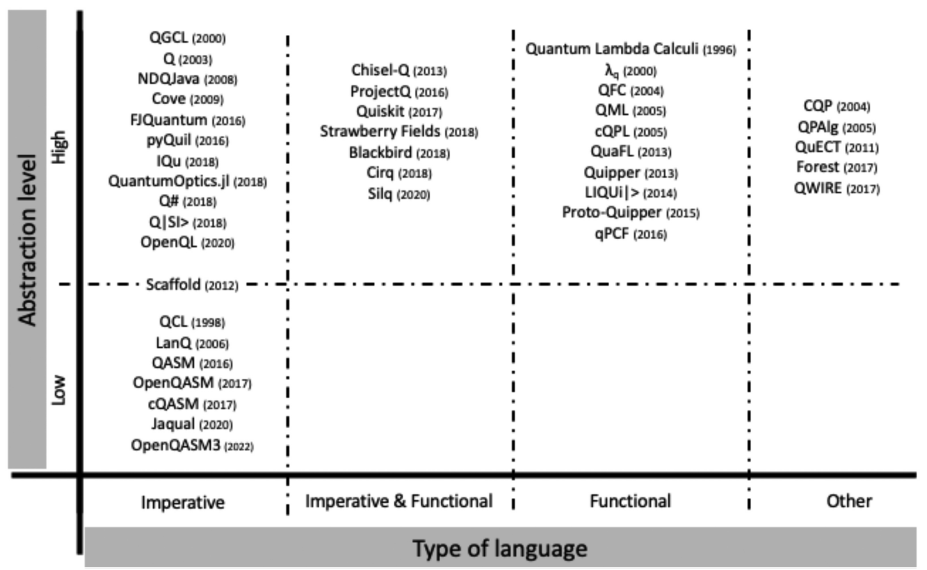
\includegraphics[width=1\linewidth]{images/quantum-programming/Quantum-Programming-Landscape.png}
    \caption{Übersicht über Quanten-Programmiersprachen nach Abstraktionsebenen und Programmierparadigmen. (Quantum Software Components and Platforms: Overview and Quality Assessment)}
    \label{fig:quantum-landscape}
\end{figure}

\paragraph{Hardwarebindung}
Die Hardwarebindung einer Quanten-Programmiersprache oder eines Frameworks beschreibt, inwieweit sie an eine bestimmte Quantenhardware-Plattform gebunden ist. Man unterscheidet zwischen Hardware-spezifisch und Hardware-unabhängig.

Hardware-Spezifische Frameworks sind für die Optimierung und Ausführung auf einer bestimmten Architektur konzipiert und optimiert. Sie nutzen die spezifischen Eigenschaften und Einschränkungen der Hardware zur Maximierung der Leistung. Beispiele hierfür sind Cirq, optimiert für Google Sycamore Hardware (https://quantumai.google/cirq) oder PyQuil, optimiert für Rigetti´s Quantum Cloud Service. (https://www.rigetti.com/what-we-build).

Hardware-unabhängige Sprachen und Frameworks sind so konzipiert, dass sie auf einer Vielzahl von Hardware-Plattformen ausgeführt werden können, oft durch die Verwendung von Zwischenrepräsentationen wie OpenQASM. Sie bieten eine große Flexibilität und Portabilität. Zu ihnen gehören unter anderem Qiskit von IBM sowie Q\# von Microsoft.

\paragraph{Quantenmodell} 
Eine weitere wesentliche Klassifikationsdimension ergibt sich aus dem zugrunde liegenden Quantenmodell. Quantencomputer können auf verschiedenen physikalischen Prinzipien und Berechnungsmodellen basieren, die sich auch in den Programmiersprachen widerspiegeln. Hierfür werden Programmiersprachen den Modellen aus \ref{programming-models} zugeordnet.

Das Gate-basierte Modell ist das dominanteste und am weitesten verbreitete Modell, bei dem Quantenalgorithmen durch Schaltkreise aus Quantengattern auf Qubits dargestellt werden. Ein Großteil der aktuellen Quantencomputer und Frameworks basieren auf diesem Modell. Beispiele für Sprachen und Frameworks sind die bereits erwähnten Qiskit, Cirq oder OpenQASM. 

Das messungsbasierte Paradigma (MBQC) führt Berechnungen durch eine Sequenz von Einzel-Qubit-Messungen auf einem vorbereiteten hochgradig verschränkten Anfangs-Cluster-Zustand durch. Die Wahl der Messbasis für jedes Qubit hängt hierbei von den Ergebnissen früherer Messungen ab. Bisher gibt es wenige produktive Frameworks, ein prominentes Beispiel ist jedoch der One-Way Quantum Computer. One-way (Einweg) ergibt sich daraus, dass jede Messung den Zustand eines Qubits zerstört und die Ressource verbraucht. Raussendorf et al. bewiesen, dass mithilfe eines zweidimensionalen Cluster-Zustands beliebige Quantenalgorithmen realisiert werden können, wodurch dieses Modell formal als äquivalent zum Schaltkreis-Modell zu sehen ist. (Measurement-based quantum computation)

Das adiabatische Paradigma nutzt Annealing zur Lösung komplexer Optimierungs- und Sampling-Probleme. Das bekannteste Beispiel hierfür ist das D-Wave Ocean SDK, das speziell für adiabatische Quantencomputer entwickelt wurde. Annealing übertrifft das Gate-Modell bei Optimierungsproblemen, da es den erheblichen Vorverarbeitungsaufwand vermeidet, der mit Gate-basierten Ansätzen verbunden ist. Darüber hinaus ist es deutlich toleranter gegenüber Fehlern und Rauschen und auf die Größe von Unternehmensproblemen skalierbar. (Optimization Performance of QA and QAOA D-Wave)

\paragraph{Zusammenfassung} 
In dieser Arbeit wurden bisher unter dem Begriff „Quanten-Programmiersprachen und -Frameworks“ sowohl formale, eigenständige Programmiersprachen als auch softwareseitige Entwicklungsumgebungen und Bibliotheken zusammengefasst, die die Programmierung, Ausführung und Analyse von Quantenalgorithmen ermöglichen.

Obwohl sich diese Systeme in Aufbau und Fokus teilweise unterscheiden, verfolgen sie das gemeinsame Ziel der Bildung einer Schnittstelle zwischen Quantenalgorithmen und deren Ausführung auf Quantenhardware oder Simulationen. Um eine systematische Vergleichbarkeit zu gewährleisten, wurden sie gemeinsam betrachtet und entsprechend ihrer funktionalen Eigenschaften klassifiziert. (Sollte ich den Teil lieber an den Anfang schreiben???)

Die folgende Tabelle fasst die Klassifizierungen verschiedener beispielhafter Quanten-Programmiersprachen und Frameworks zusammen. Die Einordnung beruht hierbei auf verschiedenen Arbeiten von (Quellen: A Survey on Available Tools and Technologies Enabling Quantum Computing | An exploratory study on the usage of quantum programming | Quantum Programming Language: A Systematic Review of Research Topic and Top Cited Languages | Quantum Software Components and Platforms: Overview and Quality Assessment)

\begin{table}[H]
\centering
\footnotesize
\begin{tabular}{|p{1cm}|p{3cm}|p{2cm}|l|l|p{2cm}|p{2cm}|}
\hline
\textbf{Jahr} & 
\textbf{Quantum-Programmiersprache / Framework} & 
\textbf{Abstraktions-level} & 
\textbf{Paradigma} & 
\textbf{Hardwarebindung} & 
\textbf{Quantenmodell} & 
\textbf{Hostsprache} \\
\hline
2017 & Qiskit & High-Level & Hybrid & IBM Q & Gate-basiert & Python \\
\hline
2018 & Cirq & High-Level & Hybrid & Google Sycamore & Gate-basiert & Python \\
\hline
2018 & Q\# & High-Level & Hybrid & ... & ...& C\# \\
\hline
1998 & QCL & Low-Level & Imperativ & ... & ... & C \\
\hline
2000 & qGCL & High-Level & Imperativ & ... & ... & Pascal \\
\hline
2003 & Q & High-Level & Imperativ & ... & ... & C++ \\
\hline
2006 & LanQ & Low-Level & Imperativ & ... & ... & C \\
\hline
2012 & Scaffold & Low-Level & Imperativ & ... & ... & C / C++ \\
\hline
2017 & OpenQASM & Low-Level & Imperativ & ... & ... & Assembly Lanaguage \\
\hline
2016 & pyQuil & High-Level & Imperativ & ... & ... & Python \\
\hline
2018 & Strawberry Fields & High-Level & Hybrid & ... & ... & Python \\
\hline
2020 & Silq & High-Level & Hybrid & ... & ... & Python \\
\hline
2020 & OpenQL & High-Level & Imperativ & ... & ... & Python, C++ \\
\hline
2022 & OpenQASM3 & Low-Level & Imperativ & ... & ... & Assembly Lanaguage \\
\hline
1996 & Quantum Lambda Calculi & High-Level & Funktional & ... & ... & Lambda Calculus \\
\hline
2005 & QML & High-Level & Funktional & ... & ... & Haskell \\
\hline
2013 & Quipper & High-Level & Funktional & ... & ... & Haskell \\
\hline
2020 & Braket SDK & High-Level & Hybrid & Amazon & ... & Python \\




\hline
\end{tabular}
\caption{Erweiterter Vergleich von Quantum-Programmiersprachen und Frameworks}
\label{tab:quantum_languages_full}
\end{table}
tbd

\subsection{Vertiefung ausgewählter Frameworks / QISKIT}

\textbf{Wie ausführlich soll ich diesen Teil machen? Alle drei Sprachen/Frameworks oder nur eins davon (Qiskit als Grundlage für nachfolgenden Teil und am weitesten verbreitete)? Wie detailliert?}
\begin{itemize}
    \item \textbf{Qiskit SDK:} Umfangreiche Bibliotheken, Simulator, Backendsteuerung
    \item \textbf{Cirq:} Framework von Google für Schaltungsdesign und Simulation
    \item \textbf{Q\#:} Domänenspezifische Sprache von Microsoft
\end{itemize}

\subsubsection{Qiskit}
\begin{itemize}
            \item Open-Source-SDK für Quanteninformatik
            \item Python-basiert
            \item Unterstützt IBM Quantum Experience Hardware
            \item Umfangreiches Ökosystem von Tools und Plugins
            
        \end{itemize}
Architktur
\begin{itemize}
    \item \textbf{Mehrschichtige Architektur}
    \begin{itemize}
        \item \textbf{Terra}: Grundlegende Funktionalität für das Arbeiten mit Quantenschaltkreisen
        \begin{itemize}
            \item Schaltkreisdarstellung und -manipulation
            \item Transpiler für Optimierung und Übersetzung
            \item Backend-Schnittstellen für Simulation und Hardware-Ausführung
        \end{itemize}
        
        \item \textbf{Aer}: Hochleistungs-Simulatoren
        \begin{itemize}
            \item Unterstützt verschiedene Simulationstypen: Zustandsvektor, Dichtematrix, Stabilisator
            \item Ermöglicht Rauschsimulation
        \end{itemize}
        
        \item \textbf{Ignis}: Werkzeuge für Charakterisierung und Fehlerminderung
        \begin{itemize}
            \item Fehlercharakterisierung und -kalibrierung
            \item Fehlerminderungstechniken
        \end{itemize}
        
        \item \textbf{Aqua}: Algorithmen für verschiedene Anwendungsbereiche
        \begin{itemize}
            \item Chemie, Finanzen, Maschinelles Lernen, Optimierung
        \end{itemize}
    \end{itemize}
    
    \item \textbf{Abstrakte und konkrete Schaltkreise}
    \begin{itemize}
        \item Abstrakte Schaltkreise: Repräsentation von Quantenalgorithmen auf hoher Abstraktionsebene
        \item Konkrete Schaltkreise: Implementierung mit Standardbibliothek von Gates
        \item OpenQASM als Zwischensprache für Quantenschaltkreise
    \end{itemize}
    
    \item \textbf{Transpiler}
    \begin{itemize}
        \item Übersetzt und optimiert Schaltkreise für die Ziel-Hardware
        \item Arbeitet in mehreren Durchläufen mit verschiedenen Passes
        \item Wichtige Passes:
        \begin{itemize}
            \item Layout-Selektion: Mapping von logischen zu physischen Qubits
            \item Routing: Einfügen von SWAP-Gates für nicht direkt verbundene Qubits
            \item Optimierung: Zusammenfassen von Gates, Entfernen unnötiger Gates
            \item Dekomposition: Zerlegung komplexer Gates in elementare Gates
        \end{itemize}
    \end{itemize}
    
    \item \textbf{Primitives}
    \begin{itemize}
        \item Grundlegende Bausteine für Quantenberechnungen
        \item \texttt{Sampler}: Stichproben aus Quantenschaltkreisen ziehen
        \item \texttt{Estimator}: Erwartungswerte von Observablen schätzen
    \end{itemize}
\end{itemize}

Besonderheiten und Anwendung

\begin{itemize}
    \item \textbf{Dynamische Schaltkreise}
    \begin{itemize}
        \item Ermöglichen klassisch kontrollierte Quantenoperationen
        \item Unterstützen Mid-Circuit-Messungen und bedingte Operationen
        \item Wichtig für adaptive Algorithmen und Fehlerkorrektur
    \end{itemize}
    
    \item \textbf{Fehlerminderung}
    \begin{itemize}
        \item Verschiedene Techniken zur Reduzierung von Hardwarefehlern
        \item Zero-Noise Extrapolation
        \item Probabilistic Error Cancellation
        \item Dynamical Decoupling
    \end{itemize}
    
    \item \textbf{Anwendungsgebiete}
    \begin{itemize}
        \item Quantenchemie und Materialwissenschaft
        \item Optimierungsprobleme
        \item Maschinelles Lernen
        \item Finanzmathematik
    \end{itemize}
    
    \item \textbf{Ökosystem und Community}
    \begin{itemize}
        \item Über 6 Millionen Installationen, 300.000 pro Monat
        \item 500+ Mitwirkende, die meisten nicht von IBM
        \item 300+ Pakete im Python Package Index (PyPI) hängen von Qiskit ab
        \item Über 2.000 wissenschaftliche Arbeiten haben Qiskit verwendet
    \end{itemize}
\end{itemize}



\section{Entwicklung von Quantenalgorithmen}

\subsection{Überblick über den Entwicklungsprozess}
\begin{itemize}
    \item Ziel: Praktische Umsetzung eines Quantenalgorithmus (End-to-End)
    \item Typische Phasen:
    \begin{itemize}
        \item Problemformulierung (z.\,B. Suche, Optimierung, Simulation)
        \item Auswahl eines geeigneten Paradigmas
        \item Abbildung auf ein Quantenmodell
        \item Wahl geeigneter Sprache / Frameworks (z.\,B. Qiskit)
        \item Implementierung, Testing, Ausführung (lokal und cloudbasiert)
    \end{itemize}
\end{itemize}

\subsection{Quantum Software Stack}

Das Quantencomputing basiert auf einem mehrschichtigen Software-Stack, mit dem abstrakte Quantenalgorithmen auf Quantenhardware übertragen und ausgeführt werden können. Eine mögliche Strukturierung eines solchen Software-Stacks ist in \autoref{fig:quantum-software-stack} abgebildet und setzt sich aus den drei Ebenen \emph{Nutzer (User Layer)}, \emph{Plattform (Platform Layer)} und \emph{Hardware (Hardware Layer)} zusammen. Jede dieser Schichten übernimmt spezifische Aufgaben innerhalb des Gesamtsystems und abstrahiert die Komplexität der darunterliegenden Ebenen.
\\
\paragraph{Nutzer}  
In der obersten Schicht werden Problemstellungen mittels Quantenalgorithmen (\autoref{basic_algorithms}) in konkreten Anwendungscode übertragen. Sie umfasst Werkzeuge und Bibliotheken, mit denen Entwickler Quantenalgorithmen und -anwendungen implementieren und für die Ausführung auf Quantenhardware vorbereiten können. Dazu gehören vor allem die in \autoref{sec:programming-languages} näher erläuterten Programmiersprachen und Entwicklungswerkzeuge (SDKs und Frameworks) wie Qiskit, Cirq oder Q\#.
\\
\paragraph{Plattform}  
Die Plattformschicht ist für die Kompilierung und Optimierung von Quantenprogrammen zuständig. Dazu gehören Compiler wie TKET oder der Qiskit Transpiler, die den Programmcode in Quantenhardware-kompatible Befehle übersetzen. Dazu zählen z.B. Gate-Dekomposition, Qubit-Zuordnung und Optimierung hinsichtlich Laufzeit und Fehlerresistenz. Auch dedizierte Software zur Fehlerkorrektur wie Riverlane kann dieser Schicht zugeordnet werden. Darüber hinaus enthält die Plattformschicht Simulatoren und Emulatoren wie Qiskit Aer oder Intel Quantum Simulator. Dabei handelt es sich um Software, die echte Quantenhardware nachbildet und so ein einfacheres Testen, Debuggen und Optimieren von Quantenanwendungen ermöglicht.
\\
\paragraph{Hardware}  
Am unteren Ende des Software-Stacks befindet sich die eigentliche Quantenhardware (Quantum Processing Unit) sowie Software für deren Verwaltung und Überwachung. Kontrollsysteme wie Quantum Machines OPX+ ermöglichen beispielsweise die Kalibrierung, Pulsgenerierung und qubitgenaue Steuerung der Hardware. Außerdem umfasst die Hardwareschicht weitere Fehlerkorrekturmechanismen.
\\
\\
Jede Schicht im Software-Stack abstrahiert technische Details der darunterliegenden Ebene und trägt zur strukturierten Entwicklung, Optimierung und Ausführung von Quantenprogrammen bei. \autocite{shehata_building_2025} \autocite{ryan_understanding_2024}

\begin{figure}[ht!]
\centering
\begin{tikzpicture}[
  layerbox/.style={
    draw,
    minimum width=6cm,
    minimum height=0.8cm,
    text centered
  }
]

\node[layerbox] (l1) at (0,  0) {Programmiersprachen};
\node[layerbox] (l2) at (0, -1) {SDKs und Frameworks};
\node[layerbox] (l3) at (0, -2) {Quantenalgorithmen};
\node[layerbox] (l4) at (0, -3) {Quantenanwendungen};

\node[layerbox] (l5) at (0, -4.5) {Simulation};
\node[layerbox] (l6) at (0, -5.5) {Kompilierung};
\node[layerbox] (l7) at (0, -6.5) {Fehlerkorrektur};

\node[layerbox] (l8) at (0, -8) {Kontrollsysteme};
\node[layerbox] (l9) at (0, -9) {Quantum Processing Unit (QPU)};

\draw[decorate, decoration={brace, amplitude=6pt, mirror}, very thick]
  ($(l1.north west) + (-0.2,0.1)$) -- ($(l4.south west) + (-0.2,-0.1)$)
  node[midway, xshift=-0.4cm, anchor=east, font=\normalsize\bfseries] {Nutzer};

\draw[decorate, decoration={brace, amplitude=6pt, mirror}, very thick]
  ($(l5.north west) + (-0.2,0.1)$) -- ($(l7.south west) + (-0.2,-0.1)$)
  node[midway, xshift=-0.4cm, anchor=east, font=\normalsize\bfseries] {\textbf{Plattform}};

\draw[decorate, decoration={brace, amplitude=6pt, mirror}, very thick]
  ($(l8.north west) + (-0.2,0.1)$) -- ($(l9.south west) + (-0.2,-0.1)$)
  node[midway, xshift=-0.4cm, anchor=east, font=\normalsize\bfseries] {\textbf{Hardware}};

\end{tikzpicture}
\caption{Struktur eines Quantum Software-Stacks \autocite{ryan_understanding_2024}}
\label{fig:quantum-software-stack}
\end{figure}

\textbf{Näher eingehen auf Compiler und Simulator?}

\subsection{Quantum Cloud Computing}

Die in der untersten Schicht des Quantum Software-Stacks befindliche Quantenhardware ist teuer in der Anschaffung und komplex zu betreiben. Das Konzept des Quantum Cloud Computing (QCC) zielt darauf ab, Endnutzern den Zugang zu Quantenhardware über Cloud-Plattformen zu erleichtern. Diese bieten Zugang zu Ressourcen, Jobmanagement und Fehlermitigation mittels abstrahierter Schnittstellen in einer skalierbaren Umgebung.

Ein zentraler Vorteil Cloud-basierter Quantenplattformen liegt in ihrer Flexibilität: Nutzer können ihre Rechenkapazitäten bedarfsgerecht skalieren, was die Bearbeitung unterschiedlich komplexer Probleme effizienter gestaltet. Außerdem ermöglichen sie das einfache Entwickeln und Testen von Quantenalgorithmen in simulierten Umgebungen, bevor diese auf echter Hardware ausgeführt werden. Dies reduziert die Einstiegshürden, da keine spezialisierte Infrastruktur oder tiefgreifende Hardwarekenntnisse notwendig sind. Da alle Nutzer auf dieselbe Plattform zugreifen, werden darüber hinaus globale Kollaboration und standardisierte Entwicklungsumgebungen begünstigt.

Zu den wichtigsten Anbietern von Quantum Cloud Plattformen zählen aktuell IBM, Amazon und Google. Ihre Plattformen IBM Quantum\footnote{IBM Quantum \url{https://quantum.ibm.com/}}, Amazon Braket\footnote{Amazon Braket \url{https://aws.amazon.com/braket/}} und Google Quantum AI\footnote{Google Quantum AI \url{https://quantumai.google/cirq/google/concepts}} sind in \autoref{tab:quantum-cloud-platforms} gegenübergestellt \autocite{trends+challenges-TODO-sync}.

\begin{table}[ht!]
\centering
\begin{tabular}{|p{2.5cm}|p{4.8cm}|p{4cm}|}
\hline
\textbf{Plattform} & \textbf{Hardware} & \textbf{Unterstützte Sprachen / SDKs} \\
\hline
IBM Quantum & Falcon, Eagle (Supraleitende Qubits) & Qiskit \\
\hline
Amazon Braket & IonQ (Ionenfallen), Rigetti (supraleitend), OQC (Photonik) & Braket SDK, PennyLane, Qiskit \\
\hline
Google Quantum AI & Sycamore (supraleitend) & Cirq \\
\hline
\end{tabular}
\caption{Vergleich führender Quantum Cloud Plattformen}
\label{tab:quantum-cloud-platforms}
\end{table}

Alle drei Plattformen bieten Cloud-basierten Zugang zu Quantenprozessoren im Pay-as-you-go-Modell, wodurch Nutzer ohne hohe Einstiegskosten reale Quantenhardware nutzen können. Dabei unterstützen alle Anbieter hybride Workflows, bei denen klassische und quantenbasierte Berechnungen kombiniert werden. Angesichts der Fehleranfälligkeit heutiger Quantenhardware integrieren alle Plattformen Mechanismen zur Fehlermitigation. Zudem sind alle Plattformen gut in ihre jeweiligen Cloud-Ökosysteme integriert (IBM Cloud, AWS, Google Cloud), um Nutzern eine nahtlose Entwicklung und Verwaltung quantenbasierter Anwendungen zu ermöglichen.

Die drei Plattformen unterscheiden sich vor allem in der Hardwareverfügbarkeit, Softwarearchitektur und ihrem Ausführungsmodell. IBM Quantum bietet exklusiv Zugang zu eigenen supraleitenden Quantenprozessoren, darunter fortschrittliche Geräte wie den 127-Qubit-Eagle. Amazon Braket hingegen fungiert als Meta-Plattform und stellt über eine einheitliche Schnittstelle Zugang zu verschiedenartigen QPUs bereit – z.B. Ionenfallen (IonQ) und supraleitende Systeme (Rigetti, OQC). Google Quantum AI verwendet ausschließlich eigene supraleitende Chips (z.B. Sycamore), die jedoch nur ausgewählten Partnern zugänglich sind. Damit bieten IBM und AWS aktuell breiteren öffentlichen Hardwarezugang, während Google auf forschungsorientierte Hardwareentwicklung mit begrenztem Zugriff setzt.

Auch auf Softwareebene gibt es Unterschiede: IBM unterstützt mit Qiskit ein umfassendes Open-Source SDK. Braket erlaubt mehr Flexibilität, indem es neben dem eigenen SDK auch Drittanbieter-Frameworks wie PennyLane unterstützt. Google verwendet Cirq – ein eher Low-Level-orientiertes SDK, das präzise Kontrolle über qubit-spezifische Details ermöglicht, insbesondere im Kontext von Machine Learning mit TensorFlow Quantum. Bei den Ausführungsmodellen bietet IBM mit Qiskit Runtime ein latenzarmes Session-Modell inklusive dynamischer Schaltungen, während Braket hybride Jobs in AWS-Containern orchestriert. Google hingegen ermöglicht primär Batch-Ausführungen über das Quantum Engine API – ohne öffentliche Hybrid-Job-Funktionalität.

Darüber hinaus gibt es weitere Plattformen wie etwa \textit{Strangeworks}, \textit{Xanadu}, \textit{Quantinuum}, \textit{IonQ} (auch über Azure Quantum) und \textit{Microsoft Azure Quantum}. Diese bieten entweder eigene Hardwaretechnologien (wie photonische QPUs bei Xanadu oder trapped-ion Systeme bei Quantinuum) oder bündeln übergreifende Multi-Backend-Zugänge mit einheitlicher API. Microsoft ermöglicht zudem tiefe Integration in klassische Azure-Dienste, während Strangeworks auf eine benutzerfreundliche Multi-Vendor-Umgebung setzt.

\subsection{Tooling und Automatisierung}
\begin{itemize}
    \item Transpiler: Anpassung an spezifisches Backend
    \item Middleware: Warteschlange, Priorisierung, Job-IDs
    \item Backend-Optimierung: z.\,B. minimale Tiefe, minimale Fehlerwahrscheinlichkeit
    \item Möglichkeit automatisierter Testausführung mit Simulator
\end{itemize}

\subsection{Praxisbeispiel: Grover-Suche mit Qiskit} 
Dieses Beispiel veranschaulicht die praktische Umsetzung des Grover-Algorithmus zur Lösung eines unstrukturierten Suchproblems. Der Algorithmus zielt darauf ab, in einem Zustandsraum mit $2^n$ Einträgen einen bestimmten, zuvor markierten Zustand mit signifikant weniger Abfragen zu identifizieren, als dies klassisch möglich wäre. Die Implementierung erfolgt auf Grundlage eines gate-basierten Quantenmodells, wobei zunächst einfache Systeme mit zwei und drei Qubits betrachtet werden.

Ausgangspunkt ist jeweils ein Qubit-Register, das durch die Anwendung von Hadamard-Gattern in eine gleichmäßige Superposition aller möglichen Zustände überführt wird. Diese Phase der Initialisierung erzeugt einen quantenmechanischen Zustand, in dem jeder mögliche Eintrag des Suchraums mit gleicher Amplitude repräsentiert ist. Der nächste Schritt besteht in der Anwendung des sogenannten Orakels, das den gesuchten Zustand durch eine Phaseninversion markiert. In der hier realisierten Version wird im Fall von zwei Qubits der Zustand $|11\rangle$ als Zielzustand definiert und durch ein einfaches CZ-Gatter identifiziert. Für die Erweiterung auf drei Qubits wird entsprechend ein mehrfach kontrolliertes Z-Gatter eingesetzt, das gezielt den Zustand $|111\rangle$ anspricht.

Im Anschluss an das Oracle kommt der sogenannte Diffusionsoperator zur Anwendung, der eine Spiegelung aller Amplituden um ihren Mittelwert bewirkt. Ziel dieses Schritts ist es, die Wahrscheinlichkeit des markierten Zustands zu verstärken, während die übrigen Zustände unterdrückt werden. Die Umsetzung erfolgt durch eine festgelegte Folge elementarer Gatter, darunter Hadamard-, X- und kontrollierte NOT-Gatter. Schon nach einer einzigen Iteration dieses Verfahrens – bei kleinen Registern in der Regel ausreichend – ist der Zielzustand in der quantenmechanischen Wahrscheinlichkeitsverteilung deutlich hervorgehoben.

Die finale Messung der Qubits erfolgt am Ende des Algorithmus. Dabei zeigt sich, dass der zuvor markierte Zustand mit hoher Wahrscheinlichkeit detektiert wird. Die experimentelle Auswertung bestätigt die theoretische Erwartung: Der Grover-Algorithmus führt zu einer gezielten Verstärkung des gewünschten Ergebnisses. Dies wird insbesondere durch die grafische Darstellung der Messhäufigkeiten deutlich, bei der der Zielzustand als klar dominanter Messwert erscheint.

Insgesamt zeigt dieses Beispiel, wie sich ein komplexer quantenmechanischer Algorithmus mit relativ einfachen Mitteln umsetzen lässt. Die Verbindung von Theorie und Praxis wird damit greifbar: Während im Kapitel Quantenalgorithmen die mathematische Grundlage gelegt wurde, bietet die hier vorgestellte Implementierung eine konkrete Anwendung und liefert gleichzeitig einen Einstieg in den praktischen Umgang mit modernen Quantenentwicklungstools.

\subsection{Implementierung und Testing mit Qiskit}
\subsubsection{Projektstruktur und Setup (Python-Umgebung, Qiskit-Installation)}

\setlength{\parindent}{0pt} % Keine Einrückung am Absatzanfang
\setlength{\parskip}{1em}   % Fügt einen vertikalen Abstand von 1em zwischen Absätzen ein

\subsubsection*{Systemanforderungen}
Die Systemanforderungen für die Implementierung und das Testing mit Qiskit sind wie folgt:
\begin{itemize}
    \item \textbf{Betriebssystem}: Windows 10 oder 11 (64-Bit)
    \item \textbf{Python-Version}: Python 3.8 bis 3.11
    \item \textbf{Arbeitsspeicher}: Mindestens 4 GB RAM (empfohlen: 8 GB oder mehr)
    \item \textbf{Festplattenspeicher}: Ca. 1--2 GB freier Speicherplatz
    \item \textbf{Internetverbindung}: Für Installation, Updates und IBM-Zugriff
\end{itemize}

\subsubsection*{Virtuelle Umgebung und Qiskit installieren}

\begin{enumerate}
    \item \textbf{Virtuelle Umgebung einrichten} 
    
Virtuelle Umgebungen helfen dabei, Abhängigkeiten eines Projekts zu isolieren und Konflikte mit anderen Projekten zu vermeiden.
    \begin{verbatim}
python -m venv C:\Users\deinBenutzername\Documents\quantum-env
    \end{verbatim}
\textit{Dieser Befehl erstellt eine neue virtuelle Python-Umgebung im angegebenen Verzeichnis, wodurch alle Projektabhängigkeiten lokal isoliert gespeichert werden. }
   

 \item \textbf{Virtuelle Umgebung aktivieren}
    \begin{verbatim}
cd C:\Users\deinBenutzername\Documents\quantum-env
.\Scripts\activate
    \end{verbatim}
\textit{Diese Befehle wechseln in das Verzeichnis der virtuellen Umgebung und aktivieren sie.  Der Prompt zeigt danach den Namen der aktiven Umgebung an, was ein Zeichen dafür ist, dass alle weiteren Befehle lokal ausgeführt werden. }
  

    \item \textbf{pip-Version prüfen}
    \begin{verbatim}
pip --version
    \end{verbatim}
\textit{Dieser Befehl überprüft, ob der Python-Paketmanager \texttt{pip} korrekt installiert und aktiviert ist.  \texttt{pip} wird im nächsten Schritt zur Installation der Pakete verwendet. }
    
\end{enumerate}

\subsubsection*{Installation der benötigten Pakete}

\begin{enumerate}
    \setcounter{enumi}{3} % Zähler für fortlaufende Liste
    \item \textbf{Qiskit installieren}
    \begin{verbatim}
pip install qiskit
    \end{verbatim}
\textit{Dieser Befehl installiert das Hauptpaket \texttt{qiskit}, das alle grundlegenden Funktionen zur Programmierung und Simulation von Quantencomputern enthält. }

    \item \textbf{Visualisierungsfunktionen hinzufügen (optional, empfohlen)}
    \begin{verbatim}
pip install qiskit[visualization]
    \end{verbatim}
\textit{Dieser Befehl installiert zusätzliche Bibliotheken zur grafischen Darstellung von Quanten-Schaltkreisen und Simulationsergebnissen, z.B. mit Matplotlib.  Dies ist notwendig bei Nutzung von Jupyter Notebook. }

    \item \textbf{IBM Runtime installieren (optional)}
    \begin{verbatim}
pip install qiskit-ibm-runtime
    \end{verbatim}
\textit{Dieser Befehl ermöglicht die Anbindung an echte Quantenhardware über IBMs Cloud-Umgebung.  Dies ist optional, aber hilfreich für fortgeschrittene Experimente. }
\end{enumerate}

\subsubsection*{Jupyter Notebook nutzen}

\begin{enumerate}
    \setcounter{enumi}{6} % Zähler für fortlaufende Liste
    \item \textbf{Jupyter installieren}
    \begin{verbatim}
pip install jupyter
    \end{verbatim}
\textit{Dieser Befehl installiert Jupyter Notebook -- eine interaktive Umgebung, in der Python-Code, Visualisierungen und Textelemente kombiniert werden können. }


    \item \textbf{Notebook starten}
    \begin{verbatim}
jupyter notebook
    \end{verbatim}
\textit{Dieser Befehl startet den Jupyter Notebook-Server und öffnet die Benutzeroberfläche im Webbrowser.  Hier können direkt interaktive Codebeispiele mit Qiskit ausgeführt werden. }

\end{enumerate}

\subsubsection{Konstruktion des Grover Circuits:}


Um den Grover Algorithmus praktisch auf eine Quantencomputer umzusetzen, wird eine konkrete Konstruktion der Schaltung benötigt. Der Algorithmus setzt sich dabei aus 4 wesentlichen Komponenten zusammen: 
\begin{enumerate}
    \item  Initialisierung: Hierbei werden die Qubits in eine gleichmäßige Superposition gebracht
    \item Oracle: Im Oracle wird der gesuchte Zustand, welcher der Grover Algorithmus identifizieren soll, ausgewählt
    \item Diffusionsoperator: Der Diffusionsoperator verstärkt den Zustand des Oracle
    \item   Messung: Abgeschlossen wird der Algorithmus mit der Messung, um das Ergebnis zu erhalten. 
\end{enumerate}

Diese 4 Schritte können beliebig für eine beliebige Anzahl an Qubits angewendet werden. Im Folgenden werden die 4 Komponenten nochmals ausführlicher beschrieben. Das Ganze erfolgt jeweils mathematisch, konzeptionell und zusätzlich noch praktisch. Für den praktischen Teil wurde ein Grover Algorithmus mit Qiskit in Jupyter Notebooks implementiert und Codeausschnitte zeigen Schritt für Schritt die praktische Umsetzung.

\subsection*{Initialisierung}
Der Startzustand aller Qubits ist $\ket{0}$. Um eine gleichverteilte Superposition über alle Basiszustände der Qubits zu erzeugen, muss für jedes der Qubits ein Hadamard-Gate ($H$) angewendet werden. Für die Anzahl $n$ Qubits ergibt sich daraus folgender Zusammenhang:
$$
|\psi_0\rangle = H^{\otimes n}|0\rangle^{\otimes n} = \frac{1}{\sqrt{2^n}} \sum_{x=0}^{2^n-1} |x\rangle
$$
Der beschriebene Zustand bildet die Grundlage für die Amplitudenverstärkung von Grovers Algorithmus. Jede Lösung hat damit zunächst dieselbe Wahrscheinlichkeit. (vgl. \citeauthor{nielsen_quantum_2010}, \citeyear{nielsen_quantum_2010}, S.257)

Mit Qiskit in Jupyter Notebooks wird zunächst die `QuantumCircuit`-Bibliothek benötigt. Anschließend kann die Initialisierung, also der Ausgangspunkt für jeden Grover-Algorithmus, wie folgt in Qiskit umgesetzt werden:
\subsection*{Beispiel für 2 Qubits:}
\begin{verbatim}
from qiskit import QuantumCircuit

# Quantenschaltung mit 2 Qubits und 2 klassischen Bits erstellen
qc = QuantumCircuit(2, 2)

# Hadamard-Gate auf jedes Qubit anwenden
qc.h([0, 1])


\end{verbatim}


Das gewählte Beispiel ist für 2 Qubits, kann jedoch, wie bereits erwähnt, für die Anzahl $n$ Qubits beliebig erweitert werden.

\subsection*{Oracle}
Der nächste Schritt in der Implementierung des Grover-Algorithmus nennt sich Oracle. Bei Oracle handelt es sich um eine unitäre Operation $U_f$, welche den gesuchten Zustand $\ket{T}$ durch eine Phaseninversion der Qubits kenntlich macht. Das bedeutet, dass in diesem Schritt immer der gesuchte Zielzustand markiert wird. Dies erlaubt im Beispiel von 2 Qubits vier verschiedene Zielzustände: "00", "01", "10" und "11".

Dieser Zusammenhang wird wie folgt beschrieben:
$$
U_f \ket{x} = (-1)^{f(x)} \ket{x}
$$
Ein ideales Oracle wird formal wie folgt beschrieben:
$$
U_f \ket{x} = \begin{cases} -\ket{x} & \text{wenn } x \text{ der gesuchte Zustand ist} \\ \ket{x} & \text{sonst} \end{cases}
$$
Für die Standardversion des Grover-Algorithmus wird der Parameter $f(x)$ in der genannten Formel gesetzt, was zu folgender Formel führt:
$$
U_f \ket{x} = (-1)^{\delta_{x,T}} \ket{x}
$$
Die daraus entstehende Inversion lässt sich als eine Reflexion des Zustandsvektors im sogenannten Hilbertraum interpretieren. (Roy et al 2022, Grover 1996)

Zum besseren Verständnis, wie das Genannte mit Qiskit in Jupyter Notebooks umgesetzt wird, hier die Fortsetzung des Beispiels für 2 Qubits. Als Beispiel wird im Folgenden nun der Zielzustand $\ket{01}$ markiert.

Standardmäßig wirkt das CZ-Gate (Controlled-Z Gate) in Qiskit auf den Zustand $\ket{11}$. Wenn man nun einen der anderen genannten Zustände markieren möchte, muss man mit NOT-Gates (X-Gates) arbeiten, welche die Qubits so transformieren, dass der gewünschte Zielzustand vor dem CZ-Gate zum Zustand $\ket{11}$ wird und nach dem CZ-Gate wieder zurücktransformiert wird.

\subsection*{Zielzustand $\ket{01}$ markieren (Beispiel):}
Um den Zustand $\ket{01}$ zu markieren, invertieren wir das erste Qubit (Index 0) mit einem X-Gate, sodass aus $\ket{0}$ ein $\ket{1}$ wird. Das zweite Qubit (Index 1) bleibt $\ket{1}$. Somit wird aus $\ket{01}$ ein $\ket{11}$. Anschließend wenden wir das CZ-Gate an und invertieren das erste Qubit wieder zurück, um den Zustand wiederherzustellen.

\begin{verbatim}
# Oracle für den Zielzustand |01> erstellen
# Qubit 0 (links) ist 0, Qubit 1 (rechts) ist 1
# Um aus |01> ein |11> zu machen, muss Qubit 0 invertiert werden (X-Gate)

# X-Gate auf Qubit 0 anwenden (0 -> 1)
qc.x(0)
# CZ-Gate anwenden (wirkt auf |11>)
qc.cz(0, 1)
# X-Gate auf Qubit 0 zurückanwenden (1 -> 0)
qc.x(0)

# Schaltung zeichnen (optional)
# qc.draw('mpl')
\end{verbatim}
Mit dieser Vorgehensweise können beliebige Zielzustände auf einfache Weise realisiert werden, und das Ganze ohne zusätzliche Hilfs-Qubits. Das funktioniert auch für die Anzahl $n$ Qubits. 
(vgl. \citeauthor{roy_deterministic_2022}, \citeyear{roy_deterministic_2022})



\subsection*{Diffusionsoperator}
Der Diffusionsoperator, welcher auch häufig „Inversion about the mean“ genannt wird, verstärkt den im Oracle markierten Zielzustand, indem er alle Amplituden am Mittelwert reflektiert. Die Definition des Diffusionsoperators ist folgende:
$$
D = 2|\psi\rangle\langle\psi| - I
$$
Dabei steht der Parameter $|\psi\rangle$ für den gleichverteilten Zustand. Das entspricht aus geometrischer Sicht einer Spiegelung im Hilbertraum. Genau diese Operation ist für die Verstärkung des im Oracle markierten Zielzustands verantwortlich. Nach jeder Grover-Iteration bewirkt sie eine Rotation des Zustandsvektors um einen festen Winkel im Unterraum von markierten und unmarkierten Zuständen. (vgl. Grover 1996, Montanaro 2016).

In unserem gewählten Beispiel mit 2 Qubits kann der Diffusionsoperator in Qiskit wie folgt umgesetzt werden:
\begin{verbatim}
grover_circuit.h([0,1])   # Rücktransformation in H-Basis
grover_circuit.z([0,1])   # Phaseninversion aller Zustände
grover_circuit.cz([0,1])  # Inversion von |00> in H-Basis
grover_circuit.h([0,1])   # Zurück in ursrüngliche Basis
\end{verbatim}

Optional kann das auch mit dem `GroverOperator` aus der Qiskit-Bibliothek gelöst werden. Dieser kapselt Oracle und Diffusion und wird wie folgt umgesetzt:
\begin{verbatim}
from qiskit.circuit.library import GroverOperator
grover_op = GroverOperator (oracle=oracle)
\end{verbatim}

\subsection*{Messung}
Der abschließende Schritt im Grover Algorithmus ist die Messung. Diese folgt nach mehreren Iterationen von Oracle und Diffusion (typischerweise $\approx \frac{\pi}{4} \sqrt{2^n}$)
\begin{verbatim}
grover_circuit.measure_all()
\end{verbatim}
Diese überführt den quantenmechanischen Zustand in einen klassischen Bitstring. 
Die Wahrscheinlichkeit, bei der Messung den markierten Zustand zu erhalten ist nun maximal. Bei Benutzung der Simulation erfolgt diese Messung häufig mehrfach in sogenannten „shots“, um eine Wahrscheinlichkeitsverteilung zu erhalten. So lässt sich die Dominanz des gesuchten Zustands gegenüber der anderen Zustände statistisch nachweisen.

Die Konstruktion des Grover-Circuits ist modular und besteht wie beschrieben aus den genannten vier klar definierten Schritten. Mithilfe von Qiskit lassen sich diese Schritte präzise implementieren, debuggen und simulieren. Das kann sowohl für die theoretische Analyse als auch für praktische Experimente auf realen Quantencomputern verwendet werden.

(vgl. \citeauthor{ibm_quantum_nodate}, \citeyear{ibm_quantum_nodate}; vgl. \citeauthor{noauthor_grovers_nodate}, \citeyear{noauthor_grovers_nodate})
\subsubsection{Ausführung auf Simulator (Qiskit Aer)}
\subsubsection{Visualisierung von Schaltkreis und Ergebnissen}

\setlength{\parindent}{0pt} % Keine Einrückung am Absatzanfang
\setlength{\parskip}{1em}   % Fügt einen vertikalen Abstand von 1em zwischen Absätzen ein

Ein zentrales Anliegen beim Verständnis und bei der Vermittlung von Quantenalgorithmen ist die Möglichkeit, deren Funktionsweise nicht nur abstrakt-mathematisch, sondern auch visuell nachvollziehen zu können. Das folgende Kapitel widmet sich der Visualisierung des Grover-Algorithmus anhand zweier Implementierungen – einmal mit zwei, einmal mit drei Qubits – unter Verwendung des Qiskit-Frameworks. Sowohl der Aufbau des Quanten-Schaltkreises als auch die Messergebnisse werden grafisch dargestellt und interpretiert.

\paragraph*{Visualisierung des Quantenschaltkreises}
\mbox{}

Für beide Varianten des Grover-Algorithmus wird der jeweilige Quanten-Schaltkreis mit der Methode QuantumCircuit.draw() visualisiert. Diese Darstellung erlaubt einen direkten Einblick in den logischen Aufbau des Algorithmus, insbesondere in die Abfolge und Wirkung der verschiedenen quantenmechanischen Operationen. Die Schaltkreise bestehen jeweils aus mehreren charakteristischen Abschnitten:
\begin{itemize}
    \item \textbf{Initialisierung:} Alle Qubits werden im Zustand $\ket{0}$    vorbereitet.
    \item \textbf{Superposition:} Durch Anwendung von Hadamard-Gattern wird eine gleichmäßige Überlagerung aller möglichen Basiszustände erzeugt.
    \item \textbf{Oracle:} Eine gezielte Phaseninversion kennzeichnet den gesuchten Zustand. Dieser Schritt implementiert die sogenannte „Markierung“ des Zielzustands.
    \item \textbf{Diffusion (Grover-Operator):} In einem weiteren Schritt wird der markierte Zustand durch Interferenz verstärkt. Dies geschieht durch Spiegelung an der Mittelwertachse aller Amplituden.
    \item \textbf{Messung:} Zum Abschluss des Algorithmus erfolgt eine Messung aller Qubits.
\end{itemize}
\noindent
Die nachstehenden Codeausschnitte zeigen, wie die Schaltkreise für beide
Varianten im Notebook erzeugt und angezeigt werden:

\begin{verbatim}
circuit.draw()
\end{verbatim}

  \begin{figure}
      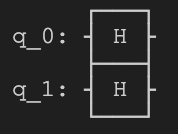
\includegraphics[width=0.25\linewidth]{circuit_superposition.png}
      \caption{Visualisierung des Schaltkreises (Superposition)}
      \label{fig:enter-label}
\end{figure}

\paragraph*{Visualisierung der Messergebnisse}
\mbox{}

Nach Ausführung des Algorithmus auf einem Quantensimulator – konkret dem QASM-Simulator von Qiskit – erfolgt die Analyse der Ergebnisse durch grafische Darstellung der Messausgänge.  Dabei wird die Methode \texttt{plot\_histogram()} verwendet, die ein Histogramm der gemessenen Zustände erzeugt.  Die Höhe der jeweiligen Balken repräsentiert die Häufigkeit (bzw. Wahrscheinlichkeit) eines bestimmten Bitmusters, das bei der Messung beobachtet wurde. 

Im Idealfall – das heißt, bei korrekter Funktionsweise des Orakels und des Grover-Operators – zeigt das Histogramm einen klar dominanten Peak beim Zielzustand.  Die Wahrscheinlichkeiten für alle anderen Zustände bleiben deutlich geringer.  Der gesuchte Zustand hebt sich somit durch quantenmechanische Verstärkung deutlich ab.  Der entsprechende Code zur Ergebnisvisualisierung lautet: 
\begin{verbatim}
plot_histogram(counts)
plt.show()
plot_histogram(counts)
plt.show()
\end{verbatim}

\begin{figure}
    \centering
    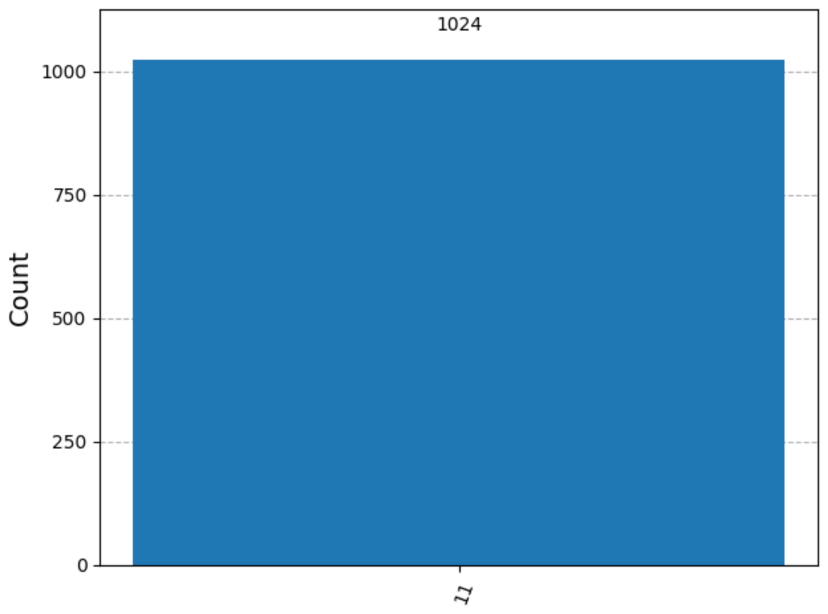
\includegraphics[width=0.75\linewidth]{Visualisierung der Messergebnisse.png}
    \caption{Visualisierung der Messergebnisse}
    \label{fig:enter-label}
\end{figure}

Die Kombination aus Schaltkreisvisualisierung und Ergebnisdarstellung bietet einen idealen Zugang zum Verständnis von Grovers Algorithmus.  Sie macht die Wirkung der einzelnen quantenlogischen Schritte nachvollziehbar und veranschaulicht das Prinzip der amplitudenbasierten Suche auf anschauliche Weise.  Solche Visualisierungen sind nicht nur didaktisch wertvoll, sondern auch essenziell für die Entwicklung und Analyse komplexerer Quantenalgorithmen in der Praxis. 

\clearpage % Fügt einen Seitenumbruch ein, um den nächsten Abschnitt auf einer neuen Seite zu beginnen

\subsubsection{Tests und Debugging-Hilfsmittel (z.\,B. Histogramme, Counts)}


\paragraph*{Tests und Debugging-Hilfsmittel}
\mbox{}

Bei der Entwicklung von Quantenalgorithmen spielt die systematische Überprüfung des Codes eine entscheidende Rolle, insbesondere im experimentellen Rahmen mit Frameworks wie Qiskit. Quantenprogramme sind nicht nur aufgrund ihrer Komplexität fehleranfällig, sondern verhalten sich auch häufig nicht intuitiv, da viele Zustände nicht direkt beobachtbar sind. Deshalb ist es essenziell, gezielt mit Tests, Zwischenergebnissen und Visualisierungen zu arbeiten, um Fehler zu erkennen und zu beheben.

\paragraph*{Schrittweise Entwicklung und Visualisierung}
\mbox{}

Im vorliegenden Notebook wurde der Grover-Algorithmus schrittweise aufgebaut, was eine erste Form des \enquote{Testens durch Design} darstellt. So wurden zunächst einzelne Operatoren und Zustände erzeugt, bevor sie in die Gesamtschaltung integriert wurden. Ein typisches Beispiel findet sich im Abschnitt zur 2-Qubit-Version:
\begin{verbatim}
def diffusion(circuit):
    circuit.h([0, 1])
    circuit.x([0, 1])
    circuit.h(1)
    circuit.cx(0, 1)
    circuit.h(1)
    circuit.x([0, 1])
    circuit.h([0, 1])
# Grover Circuit
grover_circ = QuantumCircuit(2)
grover_circ.h([0, 1])         # Superposition
oracle(grover_circ)           # Oracle anwenden
diffusion(grover_circ)        # Verstärkung
grover_circ.measure_all()
def diffusion(circuit):
    circuit.h([0, 1])
    circuit.x([0, 1])
    circuit.h(1)
    circuit.cx(0, 1)
    circuit.h(1)
    circuit.x([0, 1])
    circuit.h([0, 1])
# Grover Circuit
grover_circ = QuantumCircuit(2)
grover_circ.h([0, 1])         # Superposition
oracle(grover_circ)           # Oracle anwenden
diffusion(grover_circ)        # Verstärkung
grover_circ.measure_all()
\end{verbatim}
Durch das schrittweise Ergänzen der Gates kann bereits in frühen Phasen kontrolliert werden, ob jede Transformation wie gewünscht wirkt. Dies entspricht einem iterativen Debugging-Verfahren.

\paragraph*{Visualisierung als Debugging-Werkzeug}
\mbox{}

Wie im vorherigen Kapitel gezeigt, wird mit \texttt{draw()} der Schaltkreis visualisiert. Dies erfüllt nicht nur dokumentarische, sondern auch diagnostische Zwecke. Es kann dadurch überprüft werden, ob etwa das Oracle korrekt umgesetzt oder die Anzahl der Grover-Iterationen richtig gewählt wurde.
\subparagraph*{Beispiel:}
\begin{verbatim}
circuit.draw()
circuit.draw()
\end{verbatim}
Fehlende oder falsch platzierte Gates werden so unmittelbar sichtbar. Besonders hilfreich ist dies bei komplexeren Operatorfolgen wie in der 3-Qubit-Version.

\paragraph*{Ergebnisanalyse durch Histogramme}
\mbox{}

Ein sehr effektives Mittel zur Fehlererkennung ist die statistische Analyse der Ausgaben. Die mit \texttt{plot\_histogram()} erzeugten Verteilungen lassen Rückschlüsse auf das Verhalten des Algorithmus zu:
\begin{verbatim}
plot_histogram(result.get_counts())
plot_histogram(result.get_counts())
\end{verbatim}
Tritt der erwartete Peak beim Zielzustand nicht auf, kann dies auf einen Fehler im Oracle, in der Grover-Iteration oder in der Initialisierung hinweisen. Wurde beispielsweise ein falsches CZ-Gatter verwendet oder versehentlich eine falsche Qubit-Reihenfolge angesprochen, so verteilt sich die Wahrscheinlichkeitsmasse ungleichmäßig oder falsch.

\paragraph*{Fazit}
\mbox{}

Die Arbeit mit Quantenalgorithmen erfordert sowohl eine sorgfältige Teststrategie, klassische Softwareentwicklung aber auch eine strukturiertere Herangehensweise. Im Notebook werden bereits einfache Mittel wie Visualisierung, gezielte Zwischenschritte und Histogrammanalyse genutzt und sind eine große Hilfe beim Debugging. Für komplexere Algorithmen empfiehlt sich darüber hinaus der gezielte Einsatz von Statevector-Simulationen, Barrieren zur Strukturierung und die Ausgabe von Zwischenzuständen.

\subsection{Fazit und Ausblick}
\begin{itemize}
    \item Zusammenfassung der Entwicklungsschritte
    \item Stärken und Schwächen aktueller Toolchains
    \item Ausblick: Hybrid-Ansätze, komplexere Anwendungsfälle, Integration in klassische Softwarelandschaften
\end{itemize}

\printbibliography
uantenmechanischen System ist es jedoch nicht so einfach möglich, eine Messung durchzuführen, da ein solcher Schritt den Superpositionszustand des Qubits kollabieren ließe und damit die gespeicherte Information unter Umständen irreversibel zerstören könnte. \cite{nielsen_michael_a_and_isaac_l_chuang_quantum_2010}

Um das zu umgehen, führt man im Bereich der Quanten-Fehlerkorrektur sogenannte Syndrommessungen durch. Dabei handelt es sich um Messungen, bei denen nicht der Zustand des Qubits direkt gemessen wird, sondern nur Information über das Eintreten von Fehlern. Man misst dabei den sogenannten Stabilisator-Operator, der zu einem speziellen Quanten-Fehlerkorrekturcode gehört. Diese Operatoren definieren eine Menge erlaubter Zustände – sogenannte +1-Eigenzustände der Stabilizer-Gruppe. Tritt ein Fehler auf, so verändert sich die Eigenwertstruktur des Stabilisators. Ein Wechsel zwischen \(+1\) und \(-1\) ist zum Beispiel ein  Zeichen dafür, dass ein bestimmter Fehler passiert. \cite[Seite 444-446]{nielsen_michael_a_and_isaac_l_chuang_quantum_2010}

Die Syndrommessung erfolgt in der Praxis meist so, dass man Hilfsqubits (Ancillae) einführt, auf denen man den Stabilisator wirken lässt und so Informationen darüber erhält, was der Stabilizer auf den gekodeten Zustand angewendet hätte, ohne hierbei den gekodeten Zustand zu verändern. So lassen sich ernsthaft Fehler zum Beispiel durch die sogenannten kontrollierten Operatoren auch zu dem Hilfs-Qubit "weiterleiten" und damit dort auslesen. Dabei bleibt die gekodete Quanteninformation erhalten. Man nutzt dies dazu, das sogenannte Fehlersyndrom zu bestimmen um dann gezielt unitäre Korrektur-Operatoren durchzuführen (siehe Kapitel \ref{chap:QEC3}.). \cite[Seite 444-446]{nielsen_michael_a_and_isaac_l_chuang_quantum_2010}

Ein Schlüsselelement des fehlertoleranten Quantencomputings ist die Möglichkeit, einen Quantenzustand messen zu können, ohne dass er in seinen Ursprungszustand zu zwei Drittelwahrscheinlichkeit kollabiert. Dank dieser Fähigkeit können Codes konstruiert werden, welche die Integrität von Quanteninformation auch dann noch lange Zeit sicherstellen, wenn wiederkehrende Fehler laufend erkannt und ausgebessert werden.

\subsection{Redundanz durch Kodierung}
Quanten-Fehlerkorrektur beruht auf zentraler Idee, Quantenzustände vor Fehlern zu schützen, indem Redundanz eingefügt wird. Das bedeutet, ein einzelnes logisches Qubit wird nicht durch ein einziges physikalisches Qubit dargestellt, sondern auf mehrere physikalische Qubits verteilt. Genau durch diese zusätzliche Kodierungskapazität können Fehler eintreten, ohne dass dabei die logische Quanteninformation verloren geht.

Im Unterschied zur klassischen Fehlerkorrektur, bei der Redundanz verwendet wird (z.B. dreifache Paritätsbits), muss in der Quantenwelt solch ein Ansatz jedoch mit Bedacht gewählt werden. Denn das No-Cloning-Theorem verhindert, dass man auch einfach unbekannte Quantenzustände duplizieren kann. \cite{nielsen_michael_a_and_isaac_l_chuang_quantum_2010} Stattdessen wird die Kodierung mithilfe einer kohärenten Verschränkung mehrerer Qubits erreicht, sodass die Quanteninformation nicht in einem einzelnen Qubit, sondern in einem höherdimensionalen Unterraum des Gesamtsystems gespeichert wird.

Ein bekanntes Beispiel ist der Shor-Code, bei dem ein logisches Qubit auf neun physikalische Qubits abgebildet wird. Dieser Code schützt sowohl vor Bit-Flip- als auch vor Phase-Flip-Fehlern, indem er erst eine dreifache Kopie erstellt, um Bit-Flips zu entdecken, dann jede dieser Kopien nochmals mit einer Phase-Flip-Korrektur kodiert. \cite{shor_scheme_1995}
Ebenso gut ist der Steane-Code, der sieben Qubits zum Darstellen eines logischen Qubits verwendet und den klassischen (7, 4, 3)-Hamming-Code verwendet. \cite{Steane}

Mit Hilfe einer solchen Kodierung kann Quanteninformation in einem sogenannten Code-Raum abgelegt werden, der durch eine Gruppe von Stabilisator-Operatoren definiert ist. Tritt ein Fehler auf, so wird der Zustand in einen orthogonalen Unterraum verschoben, der außerhalb des Code-Raums liegt. Dieses Umschichten lässt sich über die Syndrommessung identifizieren – und zwar ohne, dass der ursprüngliche Zustand vermessen wird. Wesentlich ist, dass die Redundanz dabei hilft, Fehler zu lokalisieren und Korrekturoperationen durchzuführen, ohne die Quantenkohärenz zu stören.

Die Redundanz durch Kodierung ist somit die Voraussetzung für alle Quanten-Fehlerkorrekturverfahren: Denn nur indem man Information auf viele Qubits verteilt, kann man dem System Fehler \(\)verzeihen, ohne dass es aus funktionalem Zerfallen lässt.

\subsection{Fehlerzustände müssen unterscheidbar sein}
Ein entscheidendes Konzept in der Quantenfehlerkorrektur ist, dass Fehler auf einfache Weise voneinander unterscheidbar sein müssen. Nur wenn Fehler Zustände auf unterschiedliche Weise beschädigen, hat man eine Chance, festzustellen welcher der Fehler aufgetreten ist, mit dem Ziel diesen gezielt zu korrigieren ohne die Quanteninformation zu verlieren.

In der Sprache der Quanteninformatik bedeutet dies, dass die durch Fehler erstellten Zustände orthogonal zueinander sein müssen, beziehungsweise so aufgebaut, dass man durch Messung eines fehlerhaften Zustands auf den Code-Raum schließen kann. Andernfalls besteht die Gefahr, dass Fehler, die zu gleichem Messausgang führen, nicht unterschieden werden können und die Messung zu einer falschen Korrektur und dem Verlust von Information führt. \cite[Seite 449–451]{nielsen_michael_a_and_isaac_l_chuang_quantum_2010}

Dieses Konzept wird durch das sogenannte Fehlerkorrekturkriterium mathematisch präzisiert. Für eine Menge von Fehlern \(\left\{E_{i}\right\}\) , die von einem Quantencode korrigiert werden sollen, gilt:
\begin{equation}
    \left\langle\psi_{a}\right| E_{i}^{\dagger} E_{j}\left|\psi_{b}\right\rangle=C_{i j} \delta_{a b}
\end{equation}
für alle Zustände \(
    \left|\psi_{a}\right\rangle,\left|\psi_{b}\right\rangle
\)  im Code-Raum. Hierbei hängt die Konstante \(
    C_{i j}
\) vom Fehler,  nicht jedoch vom kodierten Zustand ab. Dieses Kriterium ist notwendig um sicherzustellen, dass die Wirkung eines Fehlers unabhängig von der gespeicherten Information eindeutig bestimmbar ist.

Aber aufgepasst: Wenn zwei unterschiedliche Fehler denselben Effekt auf den Code haben – also nicht unterscheidbar sind –, kann keine gezielte Korrektur erfolgen. Die Fähigkeit zur Unterscheidung solcher Fehlerzustände ist also die Voraussetzung für \textit{irgendeine} syndrombasierte Fehlerkorrektur. Nur dadurch können beispielsweise Look-Up-Tabellen oder automatische Fehlerkorrekturmechanismen sicher die \textit{einzig mögliche} Korrektur wählen.

Das Prinzip hat übrigens eine Parallele zur Konstruktion von Stabilizer-Codes, bei denen unterschiedliche Fehler unterschiedliche Syndrommuster hinterlassen. Durch geschickte Wahl der Stabilisatorgruppe kann man erreichen, dass in einem Stabilizer-Code alle Fehler innerhalb der Toleranzgrenze eindeutige Syndrome haben. \cite{gottesmann Stabilizer Codes}

\subsection{Reversibilität}
Ein entscheidendes Prinzip der Quanten-Fehlerkorrektur ist es, dass sämtliche eingesetzten Operationen im Fehlerkorrekturprozess umkehrbar sein müssen. In der Quantenmechanik entsprechen sämtliche möglichen zeitlichen Entwicklungen von isolierten Systemen unitären Transformationen – also Operationen, die völlig umkehrbar sind und keine Information vernichten. Diese Forderung gilt es auch für die Fehlerkorrektur durchzusetzen, da eine unwiderrufliche Fehlerkorrektur notwendigerweise den kodierten Quantenzustand zerstören und die Kohärenz der Quanteninformation verlieren würde. \cite[Seite 450-451]{nielsen_michael_a_and_isaac_l_chuang_quantum_2010}

Anders ausgedrückt: Wenn bei einer Kette von Ereignissen ein Fehler durch das Syndrom erkannt wurde, erfolgt ihre Korrektur durch eine bestimmte, unitäre Operation, welche uns den Fehlerzustand wieder ins Urteil des Codes zurückführt. Ist dieser Zustand erreicht, ist unser Fehler nicht nur korrigiert, sondern auch so, dass wir ihn\textbf{ kohärent rekonstruieren} können – und dies ist für weiteres Quantenrechnen und für fehlerresistente Quantenrechner notwendig.

Dieses Erfordernis der Rückkehr zur Ausgangslage besitzt auch eine sehr klare und bequeme theoretische Beschreibung: Das sogenannte Nicht-Trivialitätskriterium für Fehlerkorrektur sagt uns, dass für jede nichttriviale Fehlerwirkung \(E_i\) eine zugehörige Korrekturoperation \(R_i\) existiert, so dass 
\begin{equation}
    R_{i} E_{i}|\psi\rangle=|\psi\rangle \quad \text { für alle }|\psi\rangle \in \mathcal{C}
\end{equation}
Die Fehlererkennung und -korrektur insgesamt bildet somit einen Prozess, bei dem der Quanteninformationsträger lediglich entlang eines Umwegs durch Code-Hilfsraum entlanggeführt wird und die Logikqubit-Effektivität erhalten bleibt, um in der Lage zu sein, auch weitere Quantengatter auf diese anzuwenden.

Darum unterscheidet sich die Quanten-Fehlerkorrektur deutlich z.B. von klassischen Korrekturverfahren, welche nicht unbedingt reversibel sein müssen. In der Quanteninformatik wiederum ist Reversibilität jedoch ein \textbf{fundamentales physikalisches Prinzip}, das sowohl theoretisch als auch bei der Praxis der Implementierung beachtet werden muss.

\subsection{Fehlerlokalisierung}
Ein weiteres wichtiges Konzept, das hinter der Quanten-Fehlerkorrektur steckt, ist das der Fehlerlokalisierung. Damit ist gemeint, dass ein aufgetretener Fehler am besten so gefunden und behandelt werden kann, dass er sowohl räumlich als auch logisch eng eingegrenzt ist, und dass seine Folgen sich nicht unkontrolliert über das gesamte System ausbreiten. Nur wenn ein Fehler örtlich identifiziert und korrigiert werden kann, ist eine skalierbare und robuste Fehlerkorrektur möglich. \cite[Seite 451-452]{nielsen_michael_a_and_isaac_l_chuang_quantum_2010}

Fehler können in einem Quantencomputer verschiedene Ursprünge haben – z. B. Dekohärenz, Wechselwirkung mit der Umwelt oder Fehler bei Gates. Nach dem Prinzip der Fehlerlokalisierung sollte jeder dieser Fehler anfänglich lediglich eine begrenzte Anzahl physikalischer Qubits beeinflussen. Diese Voraussetzung soll es ermöglichen, mittels sogenannter Syndrommessungen zu erkennen, wo ein Fehler aufgetreten ist, ohne dabei den globalen Quantenzustand zu zerstören.

Dieses Konzept ist eng mit der Verwendung sogenannter lokaler Fehlerkorrektur-Codes wie z. B. topologischen Codes wie dem Surface Code verbunden. Bei diesen Codes sind die Qubits in einer regelmäßigen, zweidimensionalen Gitteranordnung angeordnet, bei der jeder Stabilizer-Operator nur Qubits betrachtet, die benachbart sind. Ein auftretender Fehler produziert ein lokales Syndrom, das sich aus den Nachbarn des fehlerhaften Qubits ergibt. Dadurch kann der Fehler nicht nur gefunden, sondern auch eingegrenzt und so gezielt korrigiert werden. \cite{Fowler et al}

Insbesondere für große, skalierbare Quantenrechner ist die Fähigkeit zur Fehlerlokalisierung essentiell: Denn ohne diese müssten sämtliche Qubits miteinander verschränkt und abgefragt werden, was einen exponentiellen Kontroll- und Ressourcenaufwand bedeuten würde. Bei lokalisierbaren Fehlern hingegen können lineare oder sogar konstante Skalierungsstrategien verfolgt werden – wodurch fehlertolerante Quantencomputer in greifbare Nähe rücken.

Zusammengefasst: Fehlerlokalisierung sorgt dafür, dass weder einzelne Fehler den gesamten Code-Raum beeinträchtigen, noch langfristige Korrekturprozesse destabilisieren. Sie ist damit eine notwendige Voraussetzung für praktische, modulare und skalierbare Quanten-Architekturen.

\subsection{Fehlerschwelle (Threshhold Theorem)}
Ein fundamentaler Mechanismus, um fehlertolerante Quantencomputer auch technisch umsetzen zu können, ist das Fehlerschwellenprinzip. Dieses besagt, dass sich Quanten-Fehlerkorrektur auf lange Sicht nur dann lohnt, wenn bei den einzelnen Qubits und Operationen die Wahrscheinlichkeit eines physikalischen Fehlers unter einem bestimmten Schwellenwert liegt, der als Fehlerschwelle bezeichnet wird. Wird die Schwelle unterschritten, so können beliebig exakte Rechnungen dadurch durchgeführt werden, dass man die Fehlerkorrektur immer wieder einsetzt – selbst wenn fortwährend physikalische Fehler passieren. \cite[Seite 454-456]{nielsen_michael_a_and_isaac_l_chuang_quantum_2010}

Dieses Prinzip wurde im Rahmen des Threshold Theorems auch rigoros bewiesen \cite{Aharonov und Ben-Or}. Das Theorem besagt, dass bei einer hinreichend kleinen Fehlerrate jedes Quanten-Computing mit beliebiger Genauigkeit durchgeführt werden kann – vorausgesetzt, es gibt genügend Redundanz und Korrekturschritte. Oder anders ausgedrückt: wenn Fehler selten genug und die Möglichkeit zur Fehlerkorrektur groß genug sind, dann können Fehler „überlebt“ werden.

Der genaue Wert der Fehlerschwelle hängt vom gewählten Code, der Architektur und der Art der Fehler ab. Er beträgt typischerweise  Wert zwischen \(
    10^{-4}
\)  und \(
    10^{-2}
\) und zählt derzeit Surface Codes zu den robustesten Verfahren. Deren experimentelle Fehlerschwelle liegt bei etwa \(1 \%\) für 
ein Gatemodell. \cite{Fowler et al.}

Von zentraler Bedeutung ist das Fehlerschwellenprinzip für die Entwicklung von Quantenhardware und -architektur, da es ermöglicht Fehler unterhalb einer beherrschbaren Schwelle und nicht als absolutes Hindernis aufzufassen. Es ist damit im Grunde eine theoretische Grundlage für das fehlertolerante Quantencomputing: Man kann Rechner auch mit unzuverlässigen Bauteilen aufbauen, solange die Wahrscheinlichkeit von Fehlern unterhalb der Fehlerschwelle liegt.

\section{Praktische Realisierung der Fehlerkorrektur}\label{chap:QEC3}

Dieses Kapitel konzentriert sich auf die praktische Umsetzung der Fehlerkorrektur.
Zuerst betrachten wir einige grundlegende Code-Beispiele, die auf den in Kapitel \ref{chap:QEC2} erläuterten Prinzipien aufbauen (Abschnitt \ref{chap:QEC3.1}). Anschließend wird der Fehlerkorrekturzyklus detailliert am Beispiel der vielversprechenden Oberflächencodes dargestellt (Abschnitt \ref{chap:QEC3.2}). Abschließend werden aktuelle Schwierigkeiten auf dem Weg zu fehlertoleranten Quantencomputern diskutiert und ein Ausblick auf zukünftige Entwicklungen gegeben (Abschnitt \ref{chap:QEC3.3}). Der Fokus liegt dabei auf Aspekten der praktischen Umsetzung sowie den damit verbundenen Problemen und Lösungen.


\subsection{Anwendung von QEC-Prinzipien: Erste Code-Beispiele}\label{chap:QEC3.1}

Wie in Abschnitt \ref{chap:QEC1} ausführlich dargestellt wurde, sind Qubits anfällig für diverse
Fehler, und wie in Abschnitt \ref{chap:QEC2} erläutert, erfordern die grundlegenden Prinzipien der
Quantenmechanik (wie das No-Cloning-Theorem und das Messproblem) spezielle
Strategien zur Fehlerkorrektur. Anstatt diese Prinzipien hier erneut zu vertiefen,
konzentrieren wir uns darauf, wie sie in ersten, einfachen Fehlerkorrekturcodes
praktisch angewendet werden. Diese Codes verdeutlichen die grundlegende Idee,
logische Information durch Kodierung über mehrere physikalische Qubits und durch
Syndrommessungen zu schützen.
Erste historische Codes demonstrieren diese Prinzipien exemplarisch. Insbesondere betrachten wir den Shor-Code (9-Qubit-Code) und den Steane-Code (7-Qubit-Code) als frühe Beispiele, sowie den einfachen 3-Qubit-Code, um die Funktionsweise und mathematischen Grundlagen der QEC zu verdeutlichen.
\cite[Seite 427-430]{nielsen_quantum_2010}\\

\paragraph{3-Qubit-Wiederholungscode (Bit-Flip Code):}
Als einfachstes Beispiel dient der 3-Qubit-Wiederholungscode, der gegen Bit-Flips schützt. Hier wird ein logisches Qubit auf drei physische Qubits verteilt, z.\,B.
\[
\lvert 0_L \rangle = \lvert 000 \rangle, \quad \lvert 1_L \rangle = \lvert 111 \rangle.
\]
Durch diese Redundanz kann ein einzelner Bitfehler erkannt werden, ohne den Logikzustand direkt zu messen. Man misst dazu sogenannte Paritätsoperatoren (Stabilisatoren), die nur verraten, ob unter den drei Qubits ein Ungleichgewicht vorliegt, aber nicht, was das logische Bit ist. Konkret prüft man, ob alle drei Qubits gleich sind (\(\lvert 000 \rangle\) oder \(\lvert 111 \rangle\)) oder ob eines abweicht. Diese Syndrommessungen liefern einen Fehlerindikator (z.\,B. welches Qubit anders ist), ohne die Superposition zu zerstören. Anschließend kann durch eine entsprechende Pauli-\(X\)-Operation der Fehler rückgängig gemacht werden.

Der 3-Qubit-Code illustriert somit die Prinzipien der Fehlererkennung und -korrektur: Die Fehler sind durch orthogonale Syndrome unterscheidbar, und die Korrekturoperation (Bit-Flip auf dem identifizierten fehlerhaften Qubit) stellt den ursprünglichen Zustand wieder her (Reversibilität). Allerdings kann dieser einfache Code nur einen Bit-Flip-Fehler korrigieren und versagt, falls zwei oder mehr Qubits gleichzeitig flippen.
\cite[Seite 430-431]{nielsen_quantum_2010}\\

Die Funktionsweise des 3-Qubit-Bitflip-Codes wird in Abbildung~1.3.1 visualisiert. 
Oben ist die Kodierung eines logischen Qubits auf drei physikalische Qubits mithilfe von CNOT-Gattern dargestellt. 
Darunter folgt eine schematische Darstellung des vollständigen Fehlerkorrekturzyklus, 
der die einzelnen Schritte von der Kodierung über die Fehlererkennung bis zur gezielten Korrektur illustriert.

\begin{center}
  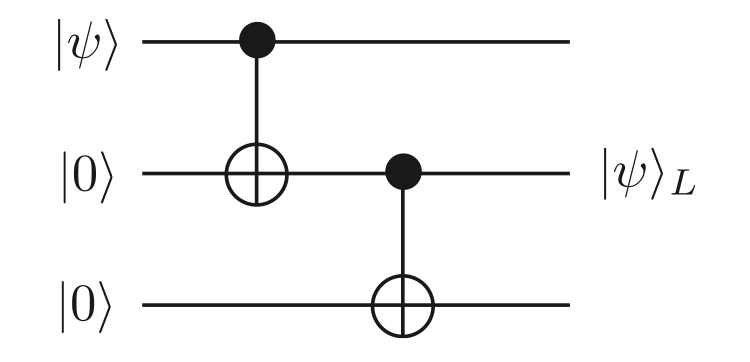
\includegraphics[width=0.5\linewidth]{images/error-correction/Abb1_BitFlipCode_1.png}
  
  \vspace{1.5em}
  
  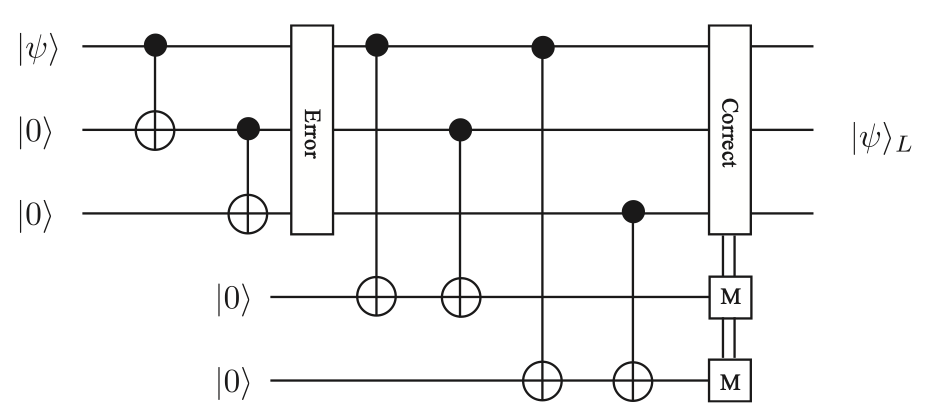
\includegraphics[width=0.5\linewidth]{images/error-correction/Abb2_BitFlipCode_2.png}
  
  \vspace{0.5em}
  
  \textbf{Abbildung 1.3.1:} Oben: Kodierung eines logischen Qubits in drei physikalische Qubits mittels CNOT-Gattern (3-Qubit-Bitflip-Code).\\
  Unten: Gesamter Zyklus aus Kodierung, Fehler, Syndrommessung und Korrektur auf Basis desselben Codes.
\end{center}
(vgl. Devitt et al., 2013, S. 7)

\paragraph{3-Qubit-Wiederholungscode (Phasenflip-Code):}\label{chap:QEC1.4}

Wie in Abschnitt~\ref{chap:QEC1.3} beschrieben, wirkt ein Phasenfehler durch Anwendung des Pauli-\(Z\)-Operators auf einen Qubit-Zustand. Dabei bleibt \(|0\rangle\) unverändert, während \(|1\rangle\) in \(-|1\rangle\) übergeht:
\[
Z(a|0\rangle + b|1\rangle) = a|0\rangle - b|1\rangle
\]
Ein solcher Vorzeichenwechsel ist in der Standardbasis \(\{|0\rangle, |1\rangle\}\) nicht direkt messbar. Betrachtet man jedoch den Zustand in der sogenannten \emph{Hadamard-Basis}, also in der Basis \(\{|+\rangle, |-\rangle\}\) mit
\[
|+\rangle = \frac{1}{\sqrt{2}}(|0\rangle + |1\rangle), \quad |-\rangle = \frac{1}{\sqrt{2}}(|0\rangle - |1\rangle),
\]
so wirkt der Phasenfehler wie ein klassischer Bitflip:
\[
Z|+\rangle = |-\rangle, \quad Z|-\rangle = |+\rangle
\]
Diesen Zusammenhang macht man sich zunutze, indem man einen Bitflip-Code in der Hadamard-Basis anwendet (vgl.\ Nielsen und Chuang, 2010, S.~430–431; Devitt et al., 2013, S.~4). Die logischen Zustände des Phasenflip-Codes lauten:
\[
|0_L\rangle = |+++\rangle, \quad |1_L\rangle = |---\rangle
\]
Ein einzelner Phasenfehler auf einem der drei Qubits kehrt den lokalen Zustand von \(|+\rangle\) zu \(|-\rangle\) um (oder umgekehrt), wodurch mithilfe von Paritätsmessungen (Syndromen) analog zum klassischen Wiederholungscode erkannt werden kann, welches Qubit betroffen ist. Eine anschließende \(Z\)-Operation korrigiert den Fehler, ohne die Superposition zu zerstören.\\

\paragraph{Shor-Code (9-Qubit-Code):}

Peter Shor entwickelte 1995 den ersten Quantenfehlerkorrekturcode, der in der Lage ist, beliebige Ein-Qubit-Fehler zu korrigieren – also sowohl Bit-Flips (\(X\)), Phasen-Flips (\(Z\)) als auch Kombinationen davon (\(Y = iXZ\)). Der sogenannte Shor-Code kombiniert zwei einfache Schutzprinzipien: eines gegen Bitfehler und eines gegen Phasenfehler.

\medskip

Das Grundprinzip besteht darin, ein einzelnes logisches Qubit auf \textbf{neun physikalische Qubits} zu verteilen. Dazu wird zunächst ein \textbf{Bit-Flip-Code} angewendet, der das Qubit dreifach wiederholt: \( |\psi\rangle \mapsto |\psi\rangle |\psi\rangle |\psi\rangle \). Das schützt gegen Bitfehler, also versehentliches Umdrehen von 0 zu 1 oder umgekehrt.

Anschließend wird jeder dieser drei Pfade durch ein \textbf{Hadamard-Gatter (\(H\))} in eine Superposition überführt. Danach folgt erneut eine dreifache Wiederholung – diesmal entlang der Zeilen. So entsteht ein Zustand, der gleichzeitig vor Phasenflips schützt. Die folgende Abbildung zeigt diesen Aufbau schematisch:

\begin{center}
    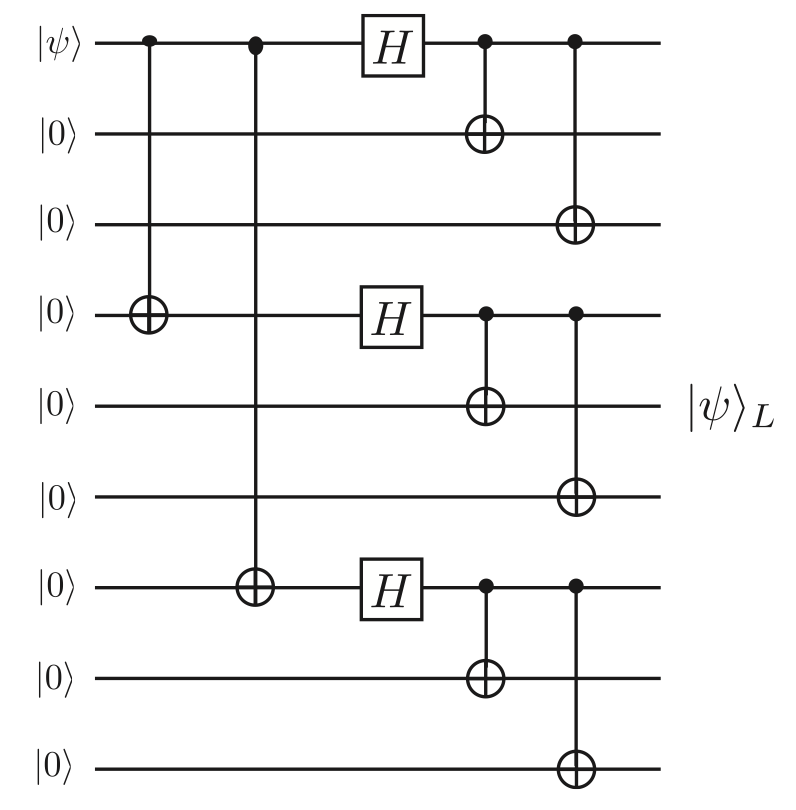
\includegraphics[width=0.5\linewidth]{images/error-correction/Abb3_ShorCode_1.png}

    \vspace{0.5em}

    \par\noindent\textbf{Abbildung 1.4.1:} Vorbereitung des Shor-Codes auf neun physikalischen Qubits. Zunächst erfolgt eine dreifache Wiederholung des Eingangszustands mithilfe von CNOT-Gattern. Anschließend wird auf jedem der drei Pfade ein Hadamard-Gatter \(H\) angewendet, das den Zustand in eine Superposition überführt. Danach folgt erneut eine dreifache Wiederholung (pro Zeile), um die Zustände \(|000\rangle \pm |111\rangle\) zu erzeugen.
\end{center}
(vgl.\ Devitt et al., 2013, S.~9)

\medskip

Formal lassen sich die kodierten logischen Zustände wie folgt schreiben:

\[
\begin{aligned}
|0_L\rangle &= \frac{1}{2\sqrt{2}} (|000\rangle + |111\rangle) \otimes (|000\rangle + |111\rangle) \otimes (|000\rangle + |111\rangle) \\
|1_L\rangle &= \frac{1}{2\sqrt{2}} (|000\rangle - |111\rangle) \otimes (|000\rangle - |111\rangle) \otimes (|000\rangle - |111\rangle)
\end{aligned}
\]

(vgl.\ Devitt et al., 2013, S.~9)

\medskip

Die Struktur ist dabei wie folgt aufgebaut: Jeder der drei Blöcke (je drei Qubits) bildet eine Superposition aus \(|000\rangle\) und \(|111\rangle\). Diese Superposition ist entweder additiv (für \(|0_L\rangle\)) oder subtraktiv (für \(|1_L\rangle\)). Dadurch entsteht ein verschränkter Gesamtzustand, der sowohl Bit- als auch Phasenfehler sichtbar macht.

\medskip

Fehlererkennung erfolgt durch Messung sogenannter \textbf{Stabilisatoren} – das sind spezielle Operatoren, die Auskunft darüber geben, ob und wo ein Fehler aufgetreten ist, ohne den gespeicherten Zustand direkt zu zerstören. So bewirkt etwa ein Phasenfehler in einem Block den Wechsel von \(|000\rangle + |111\rangle\) zu \(|000\rangle - |111\rangle\), was sich im Vorzeichen niederschlägt. Diese Änderung kann durch Syndrommessungen erkannt und der Fehler durch gezielte Anwendung eines Pauli-Operators (\(X\) oder \(Z\)) korrigiert werden.

Da ein \(Y\)-Fehler eine Kombination von \(X\)- und \(Z\)-Fehler ist, genügt es, beide Einzelfehlerarten behandeln zu können. Der Shor-Code erfüllt diese Anforderung und besitzt die Parameter \([[9, 1, 3]]\): Er kodiert ein logisches Qubit in neun physikalische und kann bis zu zwei Fehler erkennen – sowie einen davon zuverlässig korrigieren.

\medskip

Auch wenn der Code praktisch aufwendig ist, markiert er einen Meilenstein der Quanteninformationsverarbeitung: Er bewies erstmals, dass sich Quanteninformation durch geschickte Kodierung und nicht-destruktive Messung grundsätzlich vor Fehlern schützen lässt. \cite[Seite 432–434]{nielsen_quantum_2010}, (vgl.\ Devitt et al., 2013, S.~9)\\



\paragraph{Steane-Code (7-Qubit-Code):}

Der 1996 von Andrew Steane entwickelte 7-Qubit-Code ist einer der bekanntesten Quantenfehlerkorrekturcodes. Er basiert auf einem klassischen Hamming-Code und gehört zur Familie der sogenannten CSS-Codes (Calderbank-Shor-Steane). Ziel ist es, Ein-Qubit-Fehler aller Art (Bitflips \(X\), Phasenflips \(Z\) und Kombinationen daraus) mit möglichst wenigen Qubits zu erkennen und zu korrigieren.

Der Steane-Code nutzt eine clevere Strategie: Er wählt bestimmte Bitmuster aus dem klassischen \([7,4,3]\)-Hamming-Code, die sich so stark voneinander unterscheiden, dass ein einzelner Fehler sie nicht ineinander überführen kann. Diese klassischen Wörter werden anschließend in eine Superposition überführt – so entsteht echte Quantenredundanz.

Die beiden logischen Zustände \(|0_L\rangle\) und \(|1_L\rangle\) bestehen jeweils aus einer Superposition von acht solchen 7-Bit-Wörtern. Alle ausgewählten Bitmuster erfüllen spezielle Paritätsbedingungen, die es erlauben, auftretende Fehler mit sogenannten Stabilizer-Messungen zu identifizieren und zu korrigieren:
\[
\begin{aligned}
|0_L\rangle &= \frac{1}{\sqrt{8}} \big( 
|0000000\rangle + |1010101\rangle + |0110011\rangle + |1100110\rangle + {} \\
&\quad |0001111\rangle + |1011010\rangle + |0111100\rangle + |1101001\rangle \big) \\
|1_L\rangle &= \frac{1}{\sqrt{8}} \big( 
|1111111\rangle + |0101010\rangle + |1001100\rangle + |0011001\rangle + {} \\
&\quad |1110000\rangle + |0100101\rangle + |1000011\rangle + |0010110\rangle \big)
\end{aligned}
\]

Durch diese Struktur lässt sich mit nur sieben Qubits ein vollständiger Schutz gegen Ein-Qubit-Fehler erreichen – genau wie beim Shor-Code, aber effizienter.\\

Die Zustände \(|0_L\rangle\) und \(|1_L\rangle\) bestehen aus Superpositionen scheinbar willkürlicher Bitmuster wie \(|1010101\rangle\) oder \(|1100110\rangle\). Tatsächlich sind diese Muster jedoch gezielt gewählt:

\begin{itemize}
  \item Sie stammen aus dem klassischen \([7,4,3]\)-Hamming-Code, der bekannte Fehlerkorrektureigenschaften hat.
  \item Die Bitfolgen erfüllen bestimmte Paritätsbedingungen und sind so konstruiert, dass man bei einem einzelnen Bitflip noch erkennen kann, welches Bit betroffen ist.
  \item Durch die Überlagerung mehrerer solcher gültiger Codewörter (Superposition) entsteht ein Quantenfehlerkorrekturcode, der sowohl Bit- als auch Phasenfehler erkennen kann.
\end{itemize}

\noindent
Diese scheinbar komplizierten Muster sind also notwendig, um mit nur sieben Qubits vollständige Ein-Qubit-Fehlerkorrektur zu ermöglichen.
\cite[Seite 12]{devitt_qec_2013}\\

\paragraph{Ausblick auf fortgeschrittene Codes:}

Die bisher vorgestellten Codes – wie der Drei-Qubit-Code, der Shor-Code und der Steane-Code – zeigen, wie sich einzelne Bit- oder Phasenfehler gezielt erkennen und korrigieren lassen. Während sie bereits vollständige Quantenfehlerkorrektur auf einem logischen Qubit ermöglichen, stoßen sie bei wachsender Qubit-Anzahl und praktischer Realisierung an ihre Grenzen.

Für den Aufbau skalierbarer Quantencomputer werden daher weiterentwickelte Codefamilien benötigt, die neben der Korrektur beliebiger Fehler auch architektonische Vorteile bieten – etwa durch lokale Wechselwirkungen und effiziente Layouts. Ein prominentes Beispiel dafür sind die Oberflächencodes, die im folgenden Abschnitt behandelt werden. Sie beruhen auf denselben Grundprinzipien, setzen jedoch auf topologische Strukturen und fehlertolerante Operationen im Gitter.


\subsection{Der Fehlerkorrekturzyklus am Beispiel von Oberflächencodes}\label{chap:QEC3.2}

Der Oberflächencode basiert auf einem zweidimensionalen Gitter aus physikalischen Qubits, typischerweise in Form eines rechteckigen Flächenstücks (\emph{Patch}). Dabei unterscheidet man zwei Arten von Qubits: \emph{Daten-Qubits}, welche die eigentliche logische Quanteninformation tragen, und \emph{Mess-Qubits} (auch \emph{Ancilla-Qubits} genannt), die zur Fehlererkennung verwendet werden.



Man kann sich die Struktur wie ein Schachbrett vorstellen: Die Daten-Qubits liegen auf Kanten des Gitters, während die Mess-Qubits zwischen ihnen positioniert sind. Diese Mess-Qubits überwachen jeweils vier benachbarte Daten-Qubits. Dabei gibt es zwei Typen von Stabilizer-Operatoren:
\begin{itemize}
  \item \textbf{\(Z\)-Stabilizer} (auch \emph{Plaquette-Operatoren}\footnote{Plaquettes bezeichnen kleine quadratische Flächen im Gitter. Ein \(Z\)-Stabilizer wirkt auf die vier Daten-Qubits an den Ecken einer solchen Plaquette und erkennt Bitfehler.}) überprüfen die Parität in Bezug auf Bit-Flip-Fehler.
  \item \textbf{\(X\)-Stabilizer} (auch \emph{Stern-Operatoren}\footnote{Stern-Operatoren wirken auf die vier Daten-Qubits, die an einem Gitterpunkt zusammenlaufen, und erkennen Phasenfehler.}) erkennen Phasenfehler.
\end{itemize}
(vgl.\ Devitt et al., 2013, S.~28)

\begin{figure}[H]
    \centering
    \includegraphics[width=0.6\linewidth]{images/error-correction/Abb4_Oberflaechencode_1.png}
    \caption{Stabilisatorstruktur eines 2D-Oberflächen-Codes. Weiße Kreise repräsentieren Daten-Qubits. Graue Plaquettes stehen für Stabilisatoren, die jeweils auf vier benachbarte Daten-Qubits wirken: Z-Stabilisatoren (dunkel) erkennen Bit-Flip-Fehler, X-Stabilisatoren (hell) erkennen Phasenfehler (vgl.\ Kubica \cite{kubica2023}).}
    \label{fig:oberflaechencode-stabilisatoren}
\end{figure}


\paragraph{Syndrommessung und Fehlererkennung:}

Die Fehlerkorrektur erfolgt zyklisch. In jedem Zyklus werden alle \(X\)- und \(Z\)-Stabilizer gemessen. Dazu wird jedes Mess-Qubit mit den vier zugehörigen Daten-Qubits durch eine Reihe kontrollierter Gatter verschränkt, z.\,B. mit CNOT-Operationen. Nach dieser Verschaltung enthält das Mess-Qubit die Paritätsinformation: Bei \(Z\)-Stabilizern etwa, ob eine gerade oder ungerade Anzahl von \( |1\rangle \)-Zuständen in der Gruppe vorliegt. Anschließend wird das Mess-Qubit gemessen – in der \(Z\)-Basis für \(Z\)-Stabilizer und in der \(X\)-Basis für \(X\)-Stabilizer.

Das Ergebnis der Messung – 0 (Eigenwert \(+1\)) oder 1 (Eigenwert \(-1\)) – wird als \emph{Syndrom-Bit} bezeichnet. Es zeigt an, ob sich seit der letzten Messung ein Fehler ereignet hat. Wichtig ist: Diese Messungen beeinflussen den logischen Zustand nicht. Sie liefern nur Informationen über potenzielle Fehler, ohne die kodierte Quanteninformation direkt zu zerstören.

\paragraph{Decodierung und Fehlerlokalisierung:}

Die Menge aller Syndrom-Bits ergibt ein \emph{Syndrommuster}, aus dem auf die wahrscheinlichsten Fehler geschlossen werden kann. Ein einzelner Bitfehler an einem Daten-Qubit führt typischerweise dazu, dass zwei benachbarte \(Z\)-Stabilizer von 0 auf 1 wechseln. Analog dazu führt ein Phasenfehler zu Abweichungen bei zwei benachbarten \(X\)-Stabilizern.

Diese lokalen Muster bilden die Grundlage für die sogenannte \emph{Decodierung}: Ein Algorithmus analysiert die Verteilung der Fehlerhinweise und rekonstruiert den wahrscheinlichsten Fehlerpfad. Häufig wird dazu ein Graph aufgebaut, in dem Syndromabweichungen als Knoten erscheinen. Der Decoder sucht dann eine möglichst kurze Verbindung dieser Knoten – z.\,B. mithilfe eines Minimum-Weight-Perfect-Matching-Algorithmus. Auch modernere Verfahren wie Union-Find oder maschinelles Lernen kommen zum Einsatz.

Da auch Messungen fehlerhaft sein können, betrachtet man oft mehrere Zyklen hintereinander und baut einen 3D-Graphen mit der Zeitachse als dritter Dimension. Inkonstistente Syndrome über die Zeit hinweg deuten dann auf Messfehler hin.

\paragraph{Korrekturoperation:}

Nach der Decodierung steht eine Hypothese über die Art und Position der Fehler zur Verfügung. Man könnte nun direkt eine Pauli-Korrekturoperation auf das betroffene Qubit anwenden – etwa ein weiteres \(X\), um einen Bitflip rückgängig zu machen.

In der Praxis verwendet man häufig stattdessen ein sogenanntes \emph{Pauli-Frame}\footnote{Ein Pauli-Frame ist ein rein klassisches Register, in dem alle erkannten Fehler notiert werden. Die tatsächliche physische Korrektur wird dadurch vermieden und stattdessen bei der Interpretation der Messdaten berücksichtigt. So spart man potenziell fehleranfällige Operationen.}. Dabei wird die Fehlerinformation nicht physisch korrigiert, sondern nur logisch „mitgeführt“ und am Ende beim Auslesen berücksichtigt. Das spart Ressourcen und reduziert zusätzliche Fehlerquellen.

Nach Abschluss eines Fehlerkorrekturzyklus beginnt sofort der nächste – denn in einem realen Quantencomputer können ständig neue Fehler auftreten. Die kontinuierliche Wiederholung des Zyklus ermöglicht daher langfristig stabile und fehlertolerante Quanteninformation.\\

\paragraph{Einfacher Überblick: So funktioniert ein Fehlerkorrekturzyklus im Oberflächencode}Damit ein Quantencomputer trotz fehleranfälliger Qubits zuverlässig funktioniert, wird in kurzen Abständen automatisch überprüft, ob Fehler aufgetreten sind. Der Ablauf sieht dabei so aus:

\begin{enumerate}
  \item \textbf{Start:}  
  Alle Qubits werden in bekannte Anfangszustände gebracht. Die sogenannten Mess-Qubits sind bereit, nach Fehlern zu suchen.

  \item \textbf{Fehlersuche:}  
  Die Mess-Qubits „fragen“ ihre Nachbarn (die Daten-Qubits), ob alles in Ordnung ist. Aus ihren Antworten entsteht ein Muster aus Nullen und Einsen – das sogenannte \emph{Syndrom}.

  \item \textbf{Auswertung:}  
  Ein klassischer Computer schaut sich das Syndrom an und erkennt daraus, wo wahrscheinlich ein Fehler passiert ist.

  \item \textbf{Reaktion:}  
  Der Computer entscheidet, ob und wie ein Fehler korrigiert werden muss. Oft merkt man sich den Fehler einfach und berücksichtigt ihn später automatisch.

  \item \textbf{Neustart:}  
  Der nächste Zyklus beginnt sofort. So werden ständig neue Fehler früh erkannt – auch während der Quantencomputer rechnet.
\end{enumerate}

\subsection{Aktuelle H\"urden und was die Zukunft bringt}\label{chap:QEC3.3}

Trotz erster erfolgreicher Implementierungen steht die Quantenfehlerkorrektur (QEC) noch am Anfang ihrer praktischen Nutzbarkeit. Der Weg zu einem fehlertoleranten Quantencomputer ist gepflastert mit technischen und konzeptionellen Herausforderungen. In diesem Abschnitt beleuchten wir die zentralen H\"urden und geben einen Ausblick auf vielversprechende Entwicklungen.\\

\paragraph{Qubit-Qualit\"at und Fehlerschwellen} 
Ein zentrales Problem ist die Qualit\"at der physikalischen Qubits selbst. Quantenfehlerkorrektur wirkt nur, wenn die zugrunde liegenden Fehlerraten hinreichend niedrig sind. Theoretisch existiert eine Fehlerschwelle, unterhalb derer Redundanz die Zuverl\"assigkeit erh\"oht\footnote{Siehe das Threshold-Theorem in Abschnitt~\ref{chap:QEC2}}. Praktisch liegt diese Schwelle typischerweise bei Fehlerraten $\lesssim 10^{-3}$. Viele Architekturen, wie supraleitende Qubits oder Ionenfallen, erreichen in Labordemonstrationen bereits zweiqubit-Gates mit Fehlerraten im niedrigen Promillebereich, was vielversprechend ist. Doch um lange Quantenalgorithmen (z.B. Faktorisierung mit Shor bei $n=2048$) fehlerfrei auszuf\"uhren, m\"ussen logische Qubits \emph{stundenlang} koh\"arent bleiben -- ein Ziel, das nur mit sehr stabilen physikalischen Qubits erreichbar ist. Korrelierte Fehler, Leakage und seltene St\"orereignisse (z.B. kosmische Teilchen) stellen dabei zus\"atzliche Risiken dar.

\paragraph{Massiver Qubit-Overhead}
Fehlerkorrektur ist teuer: Selbst einfache Codes wie der Oberfl\"achencode ben\"otigen $O(d^2)$ physikalische Qubits f\"ur ein logisches Qubit mit Distanz $d$. Realistische Anwendungen erfordern daher \emph{Millionen} physikalischer Qubits. Derzeitige Systeme bewegen sich im Bereich von wenigen Hundert bis Tausend Qubits -- die Skalenl\"ucke ist also noch immens. Jeder weitere Qubit bringt nicht nur Nutzen, sondern auch neue Herausforderungen: Verkabelung, Kalibrierung und thermische Isolation m\"ussen f\"ur jedes Qubit mitgedacht werden.

\paragraph{Technische Limitierungen bei Kryogenik und Auslese}
Besonders supraleitende Systeme m\"ussen bei 10--20\,mK betrieben werden. Hier stoßen Forscher schnell an Grenzen: Die K\"uhlung gro\ss er Quantenprozessoren erfordert aufw\"andige Verd\"unnungsk\"uhler, und die Zahl der nach innen f\"uhrenden Kabel wird schnell zum Flaschenhals. Auch die Kontrolle \"uber klassische Elektronik ist herausfordernd: Steuereinheiten befinden sich oft au\ss erhalb des K\"uhlsystems und m\"ussen mit tausenden Kan\"alen kommunizieren -- ein thermisches und technisches Problem. Ans\"atze wie Cryo-CMOS (Steuerelektronik bei tiefen Temperaturen) werden intensiv erforscht.

\paragraph{Dekodierung: Komplex und latenzkritisch}
Selbst wenn alle Syndromdaten vorliegen, ist die Decodierung (Fehlerdiagnose und Korrekturvorschlag) ein nichttriviales Problem. Bei QEC-Zyklen im Mikrosekundenbereich und Millionen von Qubits entstehen Datenraten im Bereich hunderter Terabyte pro Sekunde. Diese m\"ussen in Echtzeit verarbeitet werden, idealerweise mit Latenzen $<1\,\mu$s. Daher ben\"otigt man spezialisierte Hardware-Decoder\footnote{Siehe z.B. Riverlane's Decodierchips oder FPGA-basierte Systeme.} und ausgekl\"ugelte Algorithmen wie Minimum Weight Matching oder Machine-Learning-gest\"utzte Ans\"atze.

\paragraph{Nicht-ideale Fehler und Modellabweichungen}
Die meisten QEC-Codes beruhen auf idealisierten Fehlermodellen (z.B. unkorrelierte, Pauli-artige Fehler). In realen Systemen treten jedoch korrelierte Fehler, Kaskadeneffekte und Leakage auf, die nicht leicht mit bestehenden Codes zu behandeln sind. Solche Abweichungen senken die effektive Fehlerschwelle und machen eine robuste Fehlerkorrektur schwieriger.\\

\paragraph{Ausblick und neue Ans\"atze}
Die Forschung reagiert mit vielf\"altigen Strategien:
\begin{itemize}
    \item \textbf{Hardwareverbesserung:} Längere Kohärenzzeiten, stabilere Qubits und besseres Materialdesign sind zentrale Entwicklungsziele.
    \item \textbf{Topologische Qubits:} Systeme wie Majorana-Moden versprechen inhärente Fehlerresistenz, sind aber noch experimentell.
    \item \textbf{Modulare Architekturen:} Mehrere kleine Qubit-Module könnten vernetzt werden, um skalierbare Systeme aufzubauen.
    \item \textbf{Neue Codes:} Quantum-LDPC-Codes, Floquet-Codes oder Color Codes bieten bessere Raten und Flexibilität, sind aber schwerer umzusetzen.
    \item \textbf{Ko-Design:} Eine enge Verzahnung von Hardware, Software und Fehlermodellen ist notwendig, um das Gesamtsystem zu optimieren.
\end{itemize}

\paragraph{Fazit} 
Die Quantenfehlerkorrektur hat sich in den letzten Jahren von einem theoretischen Konzept zu einem praktischen Forschungsfeld mit greifbaren Fortschritten entwickelt. Dennoch sind viele zentrale Herausforderungen ungel\"ost. Die kommenden Jahre werden entscheidend sein, um aus den heutigen Demonstratoren robuste, fehlertolerante Quantencomputer zu formen. Dabei ist klar: Ohne QEC ist skalierbares Quantencomputing unm\"oglich -- mit ihr aber wird es eines Tages m\"oglich sein, Probleme zu l\"osen, die klassisch unzug\"anglich bleiben.


\section{Praxisbeispiel: Ein einfacher Quantenfehlerkorrekturcode anhand des Shor-Codes: Der Shor-Code}
Wie bereits im Verlauf der vorherigen Seiten aufgezeigt sind Maßnahmen zur Fehlerkorrektur in Quantensystemen unabdingbar, um sinnvolle, verlässliche und fehlerfreie Berechnungen durchzuführen.

Das folgende Kapitel zielt darauf ab die vorher theoretisch eingeführten grundlegenden Fehler wie 
\begin{enumerate}
    \item Bitflip (Rotation um die X-Achse),
    \item Phasenflip (Rotation um die Z-Achse),
    \item Y-Flip (Rotation um die Y-Achse, also eine Kombination aus Bit- und Phasenflip)
\end{enumerate}
in einem konkreten Problemlösungssetup, dem Shor Algorithmus auf Quantencomputern, aufzuzeigen und unter Zuhilfenahme der IBM Qiskit Library anschaulich darzustellen. Zur Fehlerkorrektur innerhalb des Shor-Algorithmus wird der gleichnamige Shor Code verwendet.
Ziel dieses Beispiels ist zu Ende des Kapitels aufzuzeigen.

\subsection{Praxisbeispiel Shor-Algorithmus}
Um diesem Ziel näherzukommen wird das Beispiel des \textbf{Shor Algorithmus} zur Hand genommen. Der Shor Algorithmus ist ein Verfahren zur Berechnung von Primfaktoren sehr großer Primzahlen und ist dazu in der Lage die Periode \textbf{in polynomieller Zeit} zu finden.
Die Periode im Shor Algorithmus ist definiert als

\begin{equation}
    a^r mod N = 1
\end{equation}

Sie transformiert das in Bit-Computern schwierige Faktorisierungsproblem in ein lösbares Periodenfindungsproblem, welches durch die zuvor erläuterten QUanten-Eigenschaften der Superposition ermöglicht wird.
Während die besten klassischen Verfahren (z.B. General Number Field Sieve) subexponentielle Komplexität besitzen, findet Shor die Periode in polynomieller Zeit. Ein immenser Zugewinn.

Seine korrekte Ausführung erfordert jedoch nicht nur eine ausreichende Anzahl von Qubits, sondern auch eine hohe Gattertreue und stabile Kohärenz-eigenschaften über viele Taktzyklen hinweg. Erst durch den Einsatz von Quantenfehlerkorrektur (wie z.B durch Stabilizer- und Surface-Codes), wird der Algorithmus skalier- und praktisch anwendbar.

\subsection{Implementierung in IBM Qiskit}
\textbf{Q}uantum \textbf{I}nformation \textbf{S}cience Kit (kurz Qiskit) ist eine Software zur Visualisierung von Quantenschaltkreisen, zur Simulation von Quantencomputer-ähnlichen Umgebungen und zur Entwicklung und Ausführung von Quantenalgorithmen. Neben Simulationsoptionen bietet IBM, die Firma hinter der Open Source Software, auch Zugriff zu eigenen Quantencomputern an~\cite{qiskit}.


\subsubsection{Der Aufbau}
Zum Aufbau und zur Darstellung der Funktion des Shor-Codes wurde folgendes Beispiel-Setup implementiert:

\textbf{Der Schaltkreis} besteht aus zwei Qubit-Registern. Er zeigt die zentrale Komponente von Shor's Algorithmus zur Faktorisierung einer Zahl N. Konkret wird dadurch die Periode 
\begin{equation}
    f(x) = a^r mod N
\end{equation}
ausgerechnet und der Prozess der
Quantum Phase Estimation (QPE) dargestellt.
\\
\\
 Das obere Register (Qubits q\_0 bis q\_3) dient als Zählerregister und wird zu Beginn durch sog. Hadamard-Gates in eine Überlagerung aller möglichen Zustände versetzt, um Werte parallel untersuchen zu können.

Das untere Register (Qubits q\_4 bis q\_7) ist das sog. Funktionsregister und enthält das Ergebnis des modularen Exponenzierens.

Anschließend folgen vier kontrollierte Operationen, die jeweils --function-- realisieren. Diese Operationen sind als eigenständige Schaltkreise dargestellt (z.B. circuit-174, circuit-181 usw.) und hängen jeweils an einem der oberen Qubits. Damit führen sie die Funktion in Abhängigkeit vom Zustand des Zählerregisters aus (qiskit-doku). Diese kontrollierten modularen Berechnungen sorgen dafür, dass sich die gesuchte Periode als \textbf{Phase} in den Amplituden des Zählerregisters abbildet.

Um diese Phase messbar zu machen, wird im nächsten Schritt das sog. Inverse Quantum Fourier Transformation (iQFT) auf das Zählerregister angewendet. Diese dekodiert die phasenbehafteten Überlagerungszustände und überführt sie in ein auslesbares Interferenzmuster. Die anschließende Messung der oberen Qubits ergibt dann einen Bitstring, aus dem sich mit Hilfe klassischer Nachbearbeitung (z.B. Kettenbruchzerlegung) die Periode r rekonstruieren lässt (qiskit-doku).

Zur Simulation des Rauschens wurde ein Rauschmodell erstellt (noise\_model), das mit einer zehnprozentigen Wahrscheinlichkeit einen Bitflip Fehler auf den involvierten Qubits erzeugt und zu neunzig Prozent bei der eigentlichen Identität des Qubits verbleibt.
Zusätzlich wird der Bitflip Fehler jedes mal dann angewendet, wenn ein x- oder ein h-Gate verwendet wird.
Die "perfekt" simulierte Ausführung wird durch Zuhilfenahme des Rauschmodells also gestört und approximiert somit einen realitätsnäheren Zustand (qiskit-doku).

Damit ist das mit Qiskit's Aer-Simulator erzeugte Modell im Beispiel-Setup eine kontrollierte Fehlerquelle, deren Auswirkung durch die Anwendung im späteren Shor-Code wieder bereinigt werden soll.

\begin{figure}
    \centering
    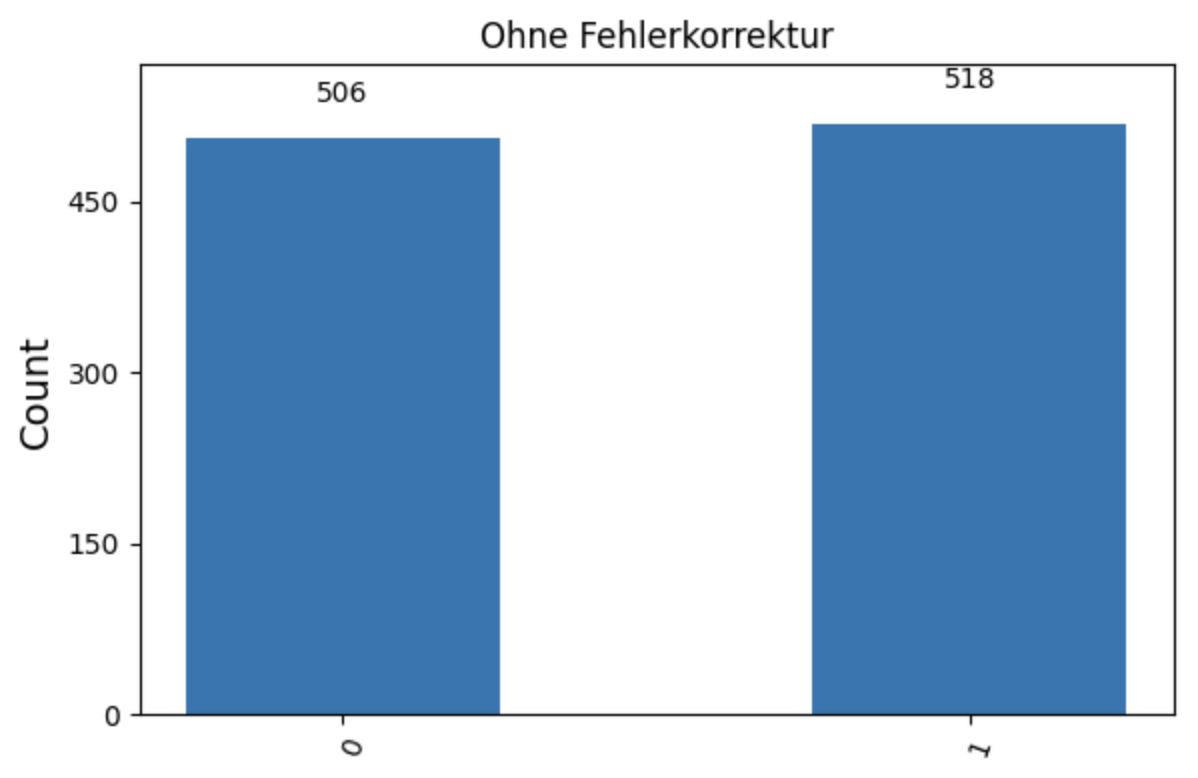
\includegraphics[width=0.75\linewidth]{images/praxis-example/result_m_ec.png}
    \caption{Durch gezieltes Verrauschen erzeugte Modifikation der Messergebnisse: 0 und 1 verschwimmen nahezu und sind in den Messergebnissen kaum noch unterscheidbar.}
    \label{fig:modified_results}
\end{figure}

Neben der Fehlersimulation 

\subsubsection{Der Shor-Code}
Um ein einzelnes logisches Qubit in einem Quantencomputer gegen Fehler zu schützen, werden beim Shor-Code insgesamt neun physikalische Qubits verwendet.

Der Grund dafür liegt in der Notwendigkeit zwei fundamentale Fehlertypen zu korrigieren: Den zuvor erläuterten Bitflip- und den Phasenflip-Fehler.

Im vorliegenden Beispiel    



Das Ergebnis ist eindeutig. Nach gezielter Fehlerkorrektur durch den Shor-Code lassen sich die Bitflip-Messergebnisse in Abbildung \ref{fig:with-error-correction} signifikant besser interpretieren, als davor. Dies zeigt sich durch die viel differenziertere Verteilung der Qubits 0 und 1, die durch die Anwendung des Shor-Codes nun korrigiert wurden.




\begin{figure}
    \centering
    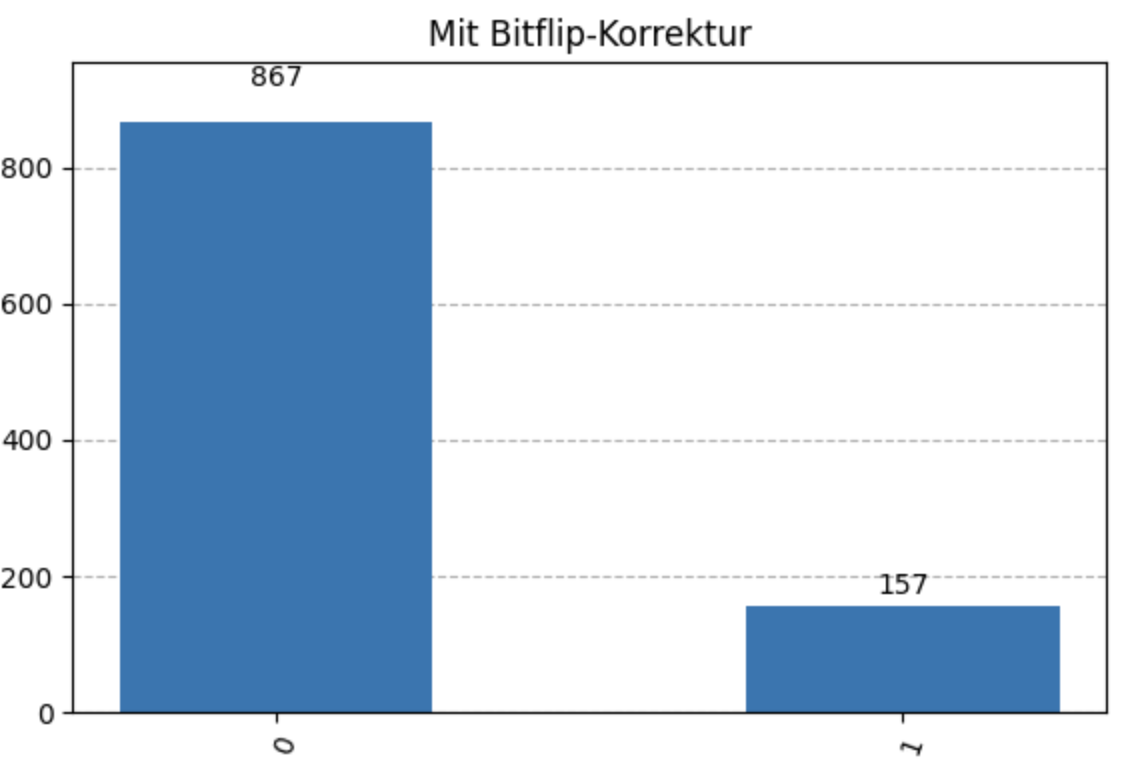
\includegraphics[width=0.75\linewidth]{images/praxis-example/result_w_ec.png}
    \caption{Caption}
    \label{fig:with-error-correction}
\end{figure}



\printbibliography
